% Nafs-Aql slide deck (Beamer). Build: ../../tools/tectonic nafs_aql_slides.tex
\documentclass[aspectratio=169,10pt]{beamer}
\usetheme{metropolis}
\usepackage[T1]{fontenc}
\usepackage{amsmath,amssymb,booktabs,array,xcolor,graphicx}
\usepackage{tikz,pgfplots}\pgfplotsset{compat=1.18}
\usetikzlibrary{arrows.meta,positioning,shapes.geometric,fit,calc,backgrounds}
% Shared palette, TikZ styles and macros for all Nafs-Aql documents
\definecolor{navy}{HTML}{1F3A5F}
\definecolor{teal}{HTML}{1B8A8F}
\definecolor{amber}{HTML}{C97D10}
\definecolor{crimson}{HTML}{B3263E}
\definecolor{violet}{HTML}{6A4C9C}
\definecolor{leaf}{HTML}{3A8F4B}
\definecolor{slate}{HTML}{5B6770}
\definecolor{sand}{HTML}{F4EFE6}
\tikzset{
  blk/.style={rounded corners=2.5pt,draw=#1!85!black,fill=#1!12,thick,align=center,
              font=\scriptsize,inner sep=3pt,minimum height=0.72cm},
  blk/.default=navy,
  sblk/.style={rounded corners=2.5pt,draw=#1!85!black,fill=#1!12,thick,align=center,
              font=\tiny,inner sep=2pt,minimum height=0.55cm},
  sblk/.default=navy,
  dm/.style={diamond,aspect=2.2,draw=amber!85!black,fill=amber!15,thick,font=\tiny,
             align=center,inner sep=0.5pt},
  st/.style={circle,draw=#1!85!black,fill=#1!15,thick,font=\scriptsize,minimum size=0.78cm,inner sep=0pt},
  st/.default=navy,
  arr/.style={-{Stealth[length=4pt,width=3pt]},thick,draw=slate},
  dsh/.style={-{Stealth[length=4pt,width=3pt]},thick,dashed,draw=slate!80},
  lab/.style={font=\tiny,fill=white,inner sep=1pt,text=black!80},
  grp/.style={rounded corners=4pt,draw=#1!60,dashed,thick,inner sep=5pt,fill=#1!4},
  grp/.default=slate,
  grplab/.style={font=\tiny\bfseries,text=#1!80!black,anchor=north west,inner sep=2pt},
  grplab/.default=slate
}
\pgfplotsset{every axis/.append style={font=\scriptsize,grid=major,grid style={black!10},
  legend style={font=\tiny,draw=none,fill=white,fill opacity=.85,text opacity=1},
  tick label style={font=\tiny},label style={font=\scriptsize}}}
% ---- shared names (single source of truth) ----
\newcommand{\Sys}{Nafs-Aql}
\newcommand{\Sone}{System~1}
\newcommand{\Stwo}{System~2}
\newcommand{\Gate}{Aql Gate}
\newcommand{\Hub}{Verifier Hub}
\newcommand{\Ledger}{Muhasaba Ledger}
\newcommand{\Distil}{Tazkiya Distillation}
\newcommand{\Mem}{Context Manager}
\newcommand{\Gw}{Rust Gateway}
\newcommand{\Harness}{Eval Harness}

\setbeamercolor{progress bar}{fg=teal,bg=teal!20}
\setbeamercolor{frametitle}{bg=navy,fg=white}
\setbeamercolor{block title}{bg=navy!85,fg=white}\setbeamercolor{block body}{bg=navy!6}
\setbeamercolor{block title alerted}{bg=crimson!85,fg=white}\setbeamercolor{block body alerted}{bg=crimson!6}
\setbeamercolor{block title example}{bg=teal!85,fg=white}\setbeamercolor{block body example}{bg=teal!7}
\setbeamerfont{block title}{size=\small}\setbeamerfont{block body}{size=\small}
\renewcommand{\Pr}{\mathbb{P}}
\newtheorem{proposition}{Proposition}
% Generated by scripts/gen_publication.py; do not edit.
\newcommand{\PhaseTwoRun}{\texttt{7ffd4442}}
\newcommand{\PhaseTwoTable}{\begin{tabular}{lrrrrr}\toprule System & $n$ & Acc. & 95\% CI & Esc. & Wall (s)\\\midrule fast\_only & 6 & 67\% & [22\%, 96\%] & 0\% & 13 \\
nafs\_aql & 6 & 100\% & [54\%, 100\%] & 33\% & 96 \\
nafs\_blind & 6 & 67\% & [22\%, 96\%] & 17\% & 133 \\
slow\_conditioned & 6 & 100\% & [54\%, 100\%] & 100\% & 319 \\
slow\_only & 6 & 100\% & [54\%, 100\%] & 100\% & 264 \\ \bottomrule\end{tabular}}
\newcommand{\BlindRouting}{50\%}
\newcommand{\GatedCostRatio}{0.36}
\newcommand{\VerifierTable}{\begin{tabular}{lrrrrr}\toprule Verifier & Correct & $r$ & Mutants & $\varphi$ & $\varphi$ upper \\\midrule code\_tests & 364 & 0.995 & 754 & 0.109 & 0.133 \\
json\_schema & 24 & 1.000 & 53 & 0.000 & 0.067 \\
judge & 23 & 1.000 & 22 & 0.045 & 0.228 \\
math\_numeric & 2000 & 1.000 & 2800 & 0.000 & 0.001 \\ \bottomrule\end{tabular}}
\newcommand{\RatesRuns}{\texttt{de66e962}, \texttt{f7991b65}, \texttt{50ff0d27}, \texttt{fd07e0a8}, \texttt{dc7168b0}}
\newcommand{\ProtocolRun}{\texttt{6c462074}}
\newcommand{\ProtocolTable}{\begin{tabular}{rrrrr}\toprule Sessions & p50 (s) & p95 (s) & p99 (s) & req/s\\\midrule 1 & 3.8 & 7.2 & 7.2 & 0.25 \\
2 & 2.7 & 4.9 & 7.2 & 0.68 \\
4 & 3.6 & 9.0 & 12.0 & 0.76 \\ \bottomrule\end{tabular}}
\newcommand{\NfrSevenRatio}{1.25}
\newcommand{\NProtocolRuns}{5}
\newcommand{\RegressionRun}{\texttt{880cdb33}}
\newcommand{\RegressionSummary}{500 items scored (done), fast-path accuracy 69\% [65\%, 73\%], mean wall 24.5\,s}
\newcommand{\ProfileCDecision}{Keep Profile A (Qwen3-1.7B) as System 1 default: accuracy 83\% vs 67\% (delta +17\%, 95\% CI [+7\%, +30\%]), mean latency 88.9 s vs 24.0 s on 30 tasks (shared machine). System 2 (Qwen3.5-4B) not evaluated at this scale; GPU scale-out (P5-T03) deferred by the user.}
\newcommand{\ProfileCTable}{\begin{tabular}{lrrrrrr}\toprule System 1 & All & Math & Code & JSON & Wall (s) & tok/s\\\midrule Qwen3-1.7B (Profile A) & 67\% & 56\% & 75\% & 83\% & 24.0 & 4.3 \\
Qwen3.5-2B (Profile C) & 83\% & 81\% & 75\% & 100\% & 88.9 & 1.9 \\ \bottomrule\end{tabular}}
\newcommand{\ProfileCDelta}{+17 points, 95\% CI [+7, +30], $n=30$}
\newcommand{\StageTable}{\begin{tabular}{llrrr}\toprule Path (replies) & Stage & Share & p50 (s) & p95 (s)\\\midrule fast (475) & System 1 draft & 98\% & 13.6 & 56.1 \\
fast (475) & verify draft & 2\% & 0.2 & 0.9 \\
deliberate (39) & System 2 deliberation & 95\% & 120.6 & 424.1 \\
deliberate (39) & judge & 3\% & 40.0 & 44.3 \\
deliberate (39) & System 1 draft & 2\% & 9.2 & 59.2 \\
deliberate (39) & probe & 1\% & 1.5 & 6.4 \\ \bottomrule\end{tabular}}
\newcommand{\EngineTable}{\begin{tabular}{lrrrr}\toprule Model stage & Calls & Prefill tok/s & Decode tok/s & Cache reuse\\\midrule System 1 draft & 485 & 53 & 7.0 & 60\% \\
cheap samples & 32 & 13 & 4.2 & 80\% \\
System 2 deliberation & 45 & 16 & 3.4 & 95\% \\ \bottomrule\end{tabular}}
\newcommand{\StageReplies}{514}
\newcommand{\EarlyEscTable}{\small\begin{tabular}{rrrrrr}\toprule $N$ & Margin & Agreement & Caught & False & Saved tok/esc.\\\midrule 32 & 0.00 & 80\% & 10/10 & 8 & 82 \\
32 & 0.02 & 95\% & 5/10 & 2 & 92 \\
32 & 0.04 & 100\% & 3/10 & 0 & 116 \\
32 & 0.15 & 100\% & 0/10 & 0 & 0 \\
48 & 0.00 & 90\% & 9/10 & 4 & 77 \\
48 & 0.02 & 98\% & 4/10 & 1 & 117 \\
48 & 0.04 & 100\% & 2/10 & 0 & 154 \\
48 & 0.15 & 100\% & 0/10 & 0 & 0 \\ \bottomrule\end{tabular}}
\newcommand{\EarlyEscSummary}{on 40 open-ended prompts, the configured rule ($N=32$, margin 0.04) agreed with the full-draft decision on 100\% of prompts, caught 3 of 10 escalations early and saved 116 draft tokens per early escalation}
\newcommand{\SecuritySummary}{26/26 security tests pass; 0 open high-severity findings}
\newcommand{\DeploySummary}{11 passed, 0 failed, 1 skipped (tool or host not available)}
\newcommand{\GatesTable}{\begin{tabular}{llp{9cm}}\toprule Gate & Status & Evidence\\\midrule G0 & pending & H7: pass; P0-T04: pending \\
G1 & fail & MVP: fail; NFR-002/004: fail \\
G2 & pending & ECE: pending; H1: pending; ER-002: pending; ER-004: pending \\
G3 & pending & TR-007: pending; OR-005: pending \\
G4 & fail & P4: pass; ER-007: pass; NFR-007: fail \\
G5 & pass & SR-006/SR-002: pass; OR-003: pass; MR-005: pass \\
G6 & pending & ER-002: pending; ER-008: pass; SR-005: pending \\ \bottomrule\end{tabular}}
\newcommand{\PolicyMapSummary}{code: the gate with the verifier for $\lambda\le0.1$, System~1 alone for $\lambda\ge0.2$; math: the gate with the verifier for $\lambda\le0.1$, System~1 alone for $\lambda\ge0.2$; structured: the gate with the verifier at every $\lambda$}
\newcommand{\PolicyMapRuns}{6}
\newcommand{\EagleTable}{\begin{tabular}{llllrr}\toprule Model & Variant & Sampling & Decode tok/s & Speed-up & Drafted tokens accepted\\\midrule System~1 & plain & greedy & 17.3 & 1.00 & -- \\
System~1 & plain & production & 18.0 & 1.00 & -- \\
System~1 & eagle3\_n4 & greedy & 18.0 & 1.04 & 52\% \\
System~1 & eagle3\_n4 & production & 17.2 & 0.95 & 49\% \\
System~1 & eagle3\_n8 & greedy & 16.0 & 0.93 & 46\% \\
System~1 & eagle3\_n8 & production & 15.4 & 0.86 & 42\% \\
System~2 & plain & greedy & 8.3 & 1.00 & -- \\
System~2 & plain & production & 7.6 & 1.00 & -- \\
System~2 & eagle3\_n4 & greedy & 8.2 & 0.99 & 46\% \\
System~2 & eagle3\_n4 & production & 7.5 & 0.99 & 46\% \\
System~2 & eagle3\_n8 & greedy & 7.3 & 0.87 & 37\% \\
System~2 & eagle3\_n8 & production & 6.9 & 0.91 & 37\% \\ \bottomrule\end{tabular}}
\newcommand{\AdaptiveExitRun}{\texttt{e7607cbb}}
\newcommand{\AdaptiveExitSummary}{with the exit: accuracy 100\%, mean wall 123\,s; without: 100\%, 220\,s ($n=11$ GSM8K items; paired $\Delta$ accuracy +0 points, 95\% CI [+0, +0])}
\newcommand{\VllmCheckSummary}{no result yet: on the day of the work the host had under 1\,GB free and the Docker VM did not start at the 7.5\,GiB the stand-in needs}
\newcommand{\QuantTable}{\begin{tabular}{lrr}\toprule Weights (Qwen3-1.7B) & Prefill tok/s & Decode tok/s\\\midrule Qwen3-1.7B-Q4\_K\_M & 81 & 15.3 \\
Qwen3-1.7B-Q4\_0 (own) & 44 & 12.2 \\
Qwen3-1.7B-IQ4\_NL (own) & 70 & 16.0 \\
Qwen3-1.7B-Q4\_K\_M (own) & 72 & 12.8 \\ \bottomrule\end{tabular}}
\newcommand{\JudgeCompare}{System~2 judge: $r=1.00$, $\varphi=0.045$ (upper 0.23); System~1 judge: $r=0.78$, $\varphi=0.27$ (upper 0.50); 23 correct and 22 seeded wrong answers}
\newcommand{\NfrSevenPooled}{median ratio 2.15 over 3 run(s) (1.25, 2.15, 2.48); fallback: document the single-session profile}

\title{Nafs-Aql}
\subtitle{A verifier-gated dual-process architecture on small Qwen models, CPU-only}
\author{Dirac R\&D Team}
\date{18 October 2026, v2.0}
\begin{document}
\maketitle

\begin{frame}{Outline}
\begin{columns}[T]
\column{.5\textwidth}
\begin{enumerate}\item Motivation and constraints\item Concept: the classical self as design metaphor\item Formal model and results\item Architecture\end{enumerate}
\column{.5\textwidth}
\begin{enumerate}\setcounter{enumi}{4}\item Implementation stack and measured feasibility\item Specification highlights\item Roadmap and gates\item \textbf{The system as built and measured results}\item Evaluation plan and the road ahead\end{enumerate}
\end{columns}
\vspace{2pt}\begin{alertblock}{Status (18 October 2026)}Phases 0--6 are implemented on the CPU reference machine and Phase~7 (CPU inference performance) was added; GPU work is deferred. Results are \emph{measured} on a shared four-core host with small samples, so they are indicative.\end{alertblock}
\end{frame}

\section{Motivation}
\begin{frame}{Why a dual-process system}
\begin{columns}[T]
\column{.55\textwidth}
\begin{block}{Observation}
Reasoning models get hard questions right by spending inference compute (long traces, many samples, verification) and waste it on easy ones. Competence is knowing when to switch.
\end{block}
\begin{block}{Constraints of this project}
\begin{itemize}\item Pretrained Qwen models, small \item CPU-only machine (4 cores, AVX2, 32\,GB) \item Unsloth for fine-tuning \item Rust web app: chat, performance tests, evaluation\end{itemize}
\end{block}
\column{.45\textwidth}
\begin{exampleblock}{What the draft had}
Twelve sound validation results, a 27B/35B GPU roster, no feasibility study, no specification, no roadmap.
\end{exampleblock}
\begin{exampleblock}{What this review delivers}
Faithful concept grounding; 17 formal results with engineering consequences; verified stack; measured CPU numbers; spec with 94 identified requirements; 7-phase roadmap with gates.
\end{exampleblock}
\end{columns}
\end{frame}

\section{Concept}
\begin{frame}{The classical self as a design metaphor}
\begin{columns}[T]
\column{.58\textwidth}
\centering\scalebox{0.78}{% Concept-to-component mapping (analogy only); width ~8.6cm
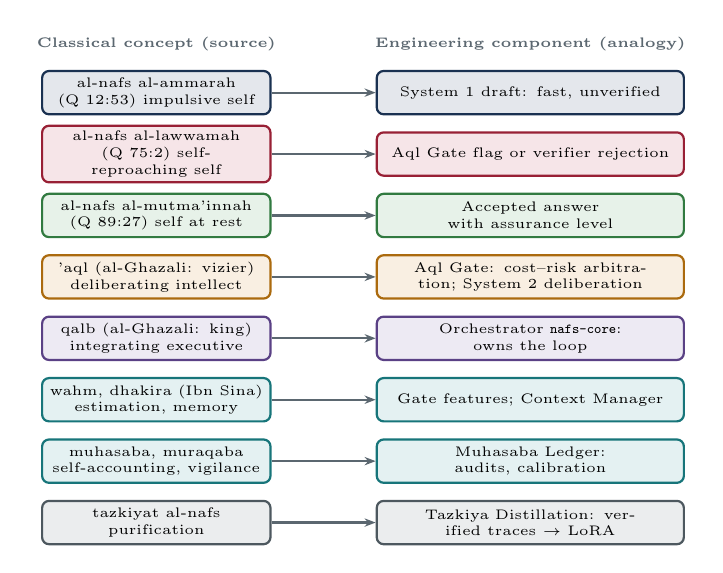
\begin{tikzpicture}[x=1cm,y=1cm]
\foreach \i/\txt/\col/\eng in {
 0/{al-nafs al-ammarah\\(Q 12:53) impulsive self}/navy/{\Sone\ draft: fast, unverified},
 1/{al-nafs al-lawwamah\\(Q 75:2) self-reproaching self}/crimson/{\Gate\ flag or verifier rejection},
 2/{al-nafs al-mutma'innah\\(Q 89:27) self at rest}/leaf/{Accepted answer with assurance level},
 3/{'aql (al-Ghazali: vizier)\\deliberating intellect}/amber/{\Gate: cost--risk arbitration; \Stwo\ deliberation},
 4/{qalb (al-Ghazali: king)\\integrating executive}/violet/{Orchestrator \texttt{nafs-core}: owns the loop},
 5/{wahm, dhakira (Ibn Sina)\\estimation, memory}/teal/{Gate features; \Mem},
 6/{muhasaba, muraqaba\\self-accounting, vigilance}/teal/{\Ledger: audits, calibration},
 7/{tazkiyat al-nafs\\purification}/slate/{\Distil: verified traces $\to$ LoRA}}
{ \node[sblk=\col,minimum width=2.9cm,text width=2.75cm] (c\i) at (0,-0.78*\i) {\txt};
  \node[sblk=\col,minimum width=3.9cm,text width=3.75cm] (e\i) at (4.75,-0.78*\i) {\eng};
  \draw[arr] (c\i)--(e\i); }
\node[font=\tiny\bfseries,text=slate] at (0,0.62) {Classical concept (source)};
\node[font=\tiny\bfseries,text=slate] at (4.75,0.62) {Engineering component (analogy)};
\end{tikzpicture}
}
\column{.42\textwidth}
\scriptsize
\begin{itemize}
\item Qur'anic stages used as mnemonics: commanding (12:53), self-reproaching (75:2), at rest (89:27)
\item al-Ghazali: heart as king, intellect as vizier, appetite and anger as soldiers
\item Ibn Sina: estimation (\emph{wahm}) and memory as internal senses
\item \emph{muhasaba}: self-correction \emph{under a standard}
\end{itemize}
\begin{alertblock}{Analogy only}No claim about the soul, consciousness or authority. The \emph{ruh}, divine inspiration and the Active Intellect are not mapped. Scholar review is a release gate.\end{alertblock}
\end{columns}
\end{frame}

\begin{frame}{One request as a bounded automaton}
\begin{columns}[T]
\column{.55\textwidth}
\centering\scalebox{0.88}{% Trace-state automaton of one request (A/L/M/T/X); width ~8.4cm
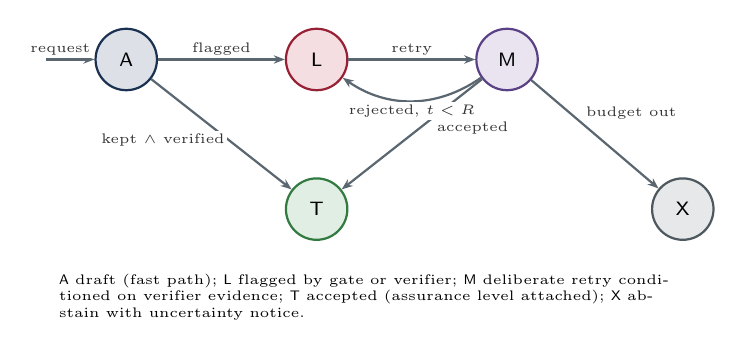
\begin{tikzpicture}[x=0.93cm,y=1cm,>=Stealth]
\node[st=navy]    (A) at (0,0)   {$\mathsf A$};
\node[st=crimson] (L) at (2.6,0) {$\mathsf L$};
\node[st=violet]  (M) at (5.2,0) {$\mathsf M$};
\node[st=leaf]    (T) at (2.6,-1.9) {$\mathsf T$};
\node[st=slate]   (X) at (7.6,-1.9) {$\mathsf X$};
\draw[arr] (-1.1,0) -- (A) node[lab,pos=0.3,above]{request};
\draw[arr] (A) -- node[lab,above]{flagged} (L);
\draw[arr] (L) -- node[lab,above]{retry} (M);
\draw[arr] (A) -- node[lab,left,pos=.55]{kept $\wedge$ verified} (T);
\draw[arr] (M) -- node[lab,below right,pos=.35]{accepted} (T);
\draw[arr] (M) to[bend left=35] node[lab,below]{rejected, $t<R$} (L);
\draw[arr] (M) -- node[lab,above right,pos=.4]{budget out} (X);
\node[font=\tiny,align=left,anchor=north west,text width=7.9cm] at (-1.05,-2.6)
 {$\mathsf A$ draft (fast path); $\mathsf L$ flagged by gate or verifier; $\mathsf M$ deliberate retry conditioned on verifier evidence;
  $\mathsf T$ accepted (assurance level attached); $\mathsf X$ abstain with uncertainty notice.};
\end{tikzpicture}
}
\column{.45\textwidth}
\small
\begin{itemize}
\item $\mathsf A$: fast draft, unverified
\item $\mathsf L$: flagged by the gate or a verifier
\item $\mathsf M$: deliberate retry on verifier evidence
\item $\mathsf T$: accepted, with an assurance level
\item $\mathsf X$: abstain with an uncertainty notice
\end{itemize}
\begin{block}{Lemma 1 (termination)}At most $1+N(R{+}1)$ model calls per request: a hard latency bound, enforced by the gateway.\end{block}
\end{columns}
\end{frame}

\section{Formal model}
\begin{frame}{Objects and objective}
\small
Task $x$, answer $y$, correctness $\kappa(x,y)$. Fast path $\pi_1$ (cost $c_1$, accuracy $p_1$); slow path $\pi_2(\cdot\mid x,b)$ with thinking budget $b$; verifier with true-accept $r$ and false-accept $\varphi$; gate $\gamma(s)$ on features $s$; loss $L$ per wrong answer, $L_a$ per abstention, price $\lambda$ per cost unit.
\begin{equation*}
\min_{\gamma,b,N,R}\ \mathbb E_x\big[L\,\Pr[\text{wrong}]+L_a\,\Pr[\text{abstain}]+\lambda\,\mathbb E[\text{cost}]\big]
\end{equation*}
\begin{columns}[T]
\column{.5\textwidth}
\begin{block}{Labels}\textbf{[exact]} no further hypotheses; \textbf{[strong]} needs an empirical check; \textbf{[conjecture]} scheduled hypothesis.\end{block}
\column{.5\textwidth}
\begin{exampleblock}{Rule}Every result ends with an engineering consequence: a parameter, an algorithm or a gate in the specification.\end{exampleblock}
\end{columns}
\end{frame}

\begin{frame}{Theorem 1: precision is bounded by the verifier}
\begin{columns}[T]
\column{.5\textwidth}
\begin{theorem}[Verified-return precision, exact]
$\rho(p)=\Pr[\text{wrong}\mid\text{accepted}]=\dfrac{\varphi(1-p)}{\varphi(1-p)+rp}$, and $\rho\le\varepsilon\iff\varphi\le\dfrac{\varepsilon rp}{(1-\varepsilon)(1-p)}$.
\end{theorem}
\small Hard tasks ($p=0.1$), 1\% target: $\varphi\le1.1\times10^{-3}$. With $\varphi=0.02$: $\rho=15.5\%$.
\begin{alertblock}{Consequence}Exact verifiers carry the safety case. Each verifier publishes $(r,\varphi)$ from mutation testing (FR-032); consensus is a flag, not a verifier.\end{alertblock}
\column{.5\textwidth}
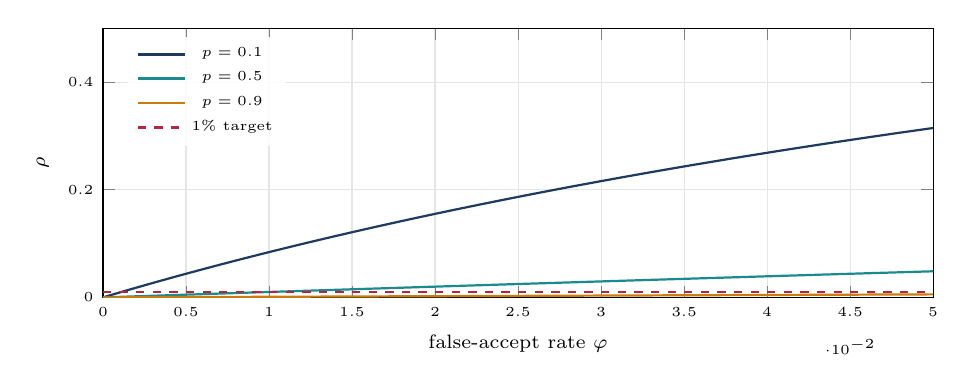
\begin{tikzpicture}
\begin{axis}[width=\linewidth,height=5cm,xlabel={false-accept rate $\varphi$},ylabel={$\rho$},xmin=0,xmax=0.05,ymin=0,ymax=0.5,legend pos=north west]
\addplot[navy,thick,domain=0:0.05,samples=60]{x*0.9/(x*0.9+0.098)};\addlegendentry{$p=0.1$}
\addplot[teal,thick,domain=0:0.05,samples=60]{x*0.5/(x*0.5+0.49)};\addlegendentry{$p=0.5$}
\addplot[amber,thick,domain=0:0.05,samples=60]{x*0.1/(x*0.1+0.882)};\addlegendentry{$p=0.9$}
\addplot[crimson,dashed,thick]coordinates{(0,0.01)(0.05,0.01)};\addlegendentry{1\% target}
\end{axis}
\end{tikzpicture}
\end{columns}
\end{frame}

\begin{frame}{Theorem 2: the gate is a derived threshold, not a tuned one}
\begin{columns}[T]
\column{.52\textwidth}
\begin{theorem}[Optimal gate, exact]
With $e_1(s)=\Pr[\text{fast wrong}\mid s]$, $e_2(s)$ the error after escalation and $\Delta c(s)$ the extra cost, escalate iff
$$L\big(e_1(s)-e_2(s)\big)>\lambda\,\Delta c(s).$$
Under a budget, the rule is a threshold on $(e_1-e_2)/\Delta c$ (Neyman--Pearson).
\end{theorem}
\begin{block}{Proposition 1 (price of miscalibration)}Estimation error $\epsilon$ on $\hat e_1$ costs at most $L\epsilon$ per request: the ECE target 0.05 (NFR-020) is a regret bound.\end{block}
\column{.48\textwidth}
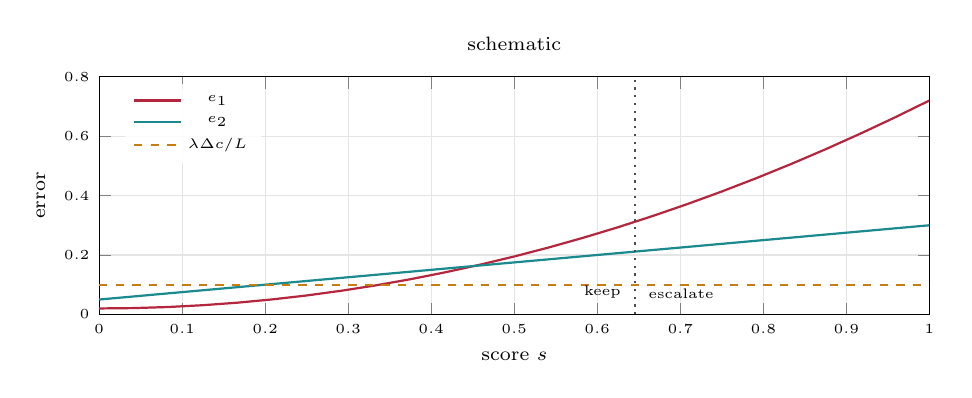
\begin{tikzpicture}
\begin{axis}[width=\linewidth,height=4.6cm,xlabel={score $s$},ylabel={error},xmin=0,xmax=1,ymin=0,ymax=0.8,legend pos=north west,title={\scriptsize schematic}]
\addplot[crimson,thick,domain=0:1]{0.02+0.7*x^2};\addlegendentry{$e_1$}
\addplot[teal,thick,domain=0:1]{0.05+0.25*x};\addlegendentry{$e_2$}
\addplot[amber,dashed,thick]coordinates{(0,0.1)(1,0.1)};\addlegendentry{$\lambda\Delta c/L$}
\addplot[black!70,dotted,thick]coordinates{(0.645,0)(0.645,0.8)};
\node[font=\tiny,anchor=south west] at (axis cs:0.65,0.02){escalate};
\node[font=\tiny,anchor=south east] at (axis cs:0.64,0.02){keep};
\end{axis}
\end{tikzpicture}
\scriptsize Same rule as Chow's reject option and the expected value of control; the only tunable is $\lambda$, the ``speed--care'' slider (Prop.\,2).
\end{columns}
\end{frame}

\begin{frame}{Theorem 3 and Proposition 3: sampling buys coverage; stopping is a Beta rule}
\begin{columns}[T]
\column{.5\textwidth}
\begin{theorem}[Coverage, exact]
Draw-verify-stop with acceptance probability $a$: coverage $1-(1-a)^M$, expected draws $(1-(1-a)^M)/a$, and the error of an accepted answer is $\rho(q)$ \emph{for every} $M$.
\end{theorem}
\begin{proposition}[Optimal cap, strong]
With $a\sim\mathrm{Beta}(\alpha,\beta)$, draw again iff $\frac{\alpha}{\alpha+\beta+m}L_a>c_p$ (monotone case), so
$M^\star=\lceil\alpha L_a/c_p-\alpha-\beta\rceil$.
\end{proposition}
\column{.5\textwidth}
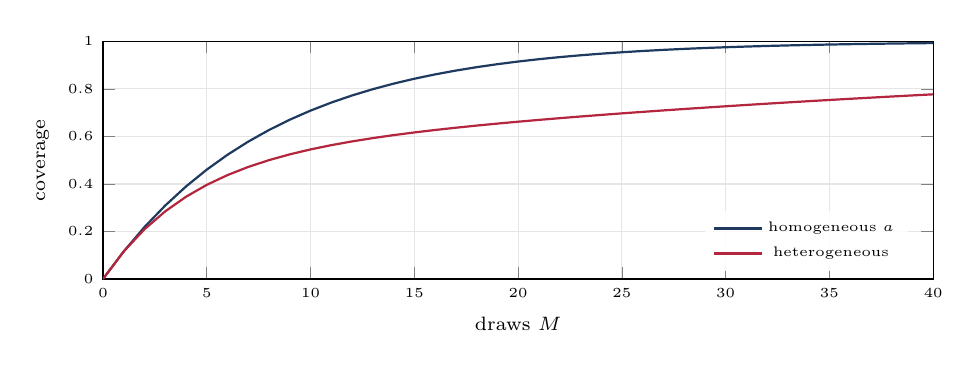
\begin{tikzpicture}
\begin{axis}[width=\linewidth,height=4.6cm,xlabel={draws $M$},ylabel={coverage},xmin=0,xmax=40,ymin=0,ymax=1,legend pos=south east]
\addplot[navy,thick,domain=0:40,samples=41]{1-(0.884)^x};\addlegendentry{homogeneous $a$}
\addplot[crimson,thick,domain=0:40,samples=41]{1-0.5*(0.788)^x-0.5*(0.98)^x};\addlegendentry{heterogeneous}
\end{axis}
\end{tikzpicture}
\begin{alertblock}{Consequence}$N$ and $R$ per domain come from the Phase-0 Beta fit and the cost ratio $c_p/L_a$ (FR-021); heterogeneity of $a$ is measured, not averaged.\end{alertblock}
\end{columns}
\end{frame}

\begin{frame}{Theorems 4 and 5: the self-monitoring loop must be verifier-gated}
\begin{columns}[T]
\column{.5\textwidth}
\begin{theorem}[Unverified refinement, strong]
If a refinement fixes a wrong answer w.p.\ $u$ and breaks a right one w.p.\ $d$, then $q_t=q^\star+(q_0-q^\star)(1-u-d)^t$ with $q^\star=u/(u+d)$: iterating \emph{harms} whenever $q_0>q^\star$.
\end{theorem}
\begin{theorem}[Verifier-gated loop, exact]
Accepting only verifier passes gives $\Pr[\text{accepted wrong}]\le\varphi\,\mathbb E[T]$ and conditional error within $[\min_t\rho(q_t),\max_t\rho(q_t)]$, independent of $(u,d)$.
\end{theorem}
\column{.5\textwidth}
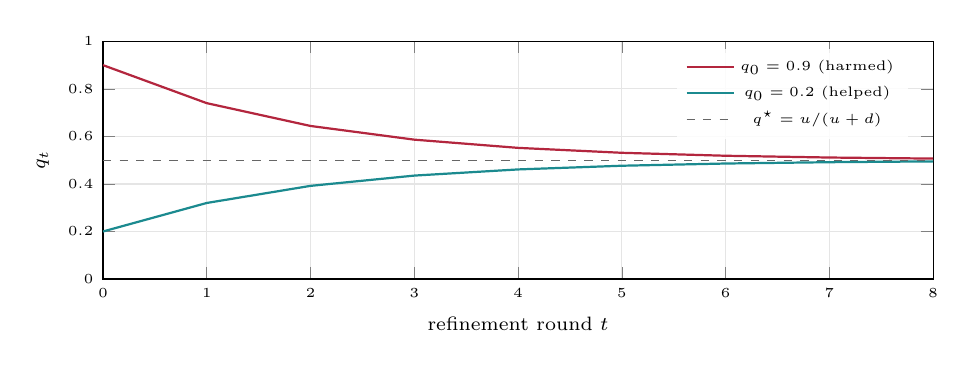
\begin{tikzpicture}
\begin{axis}[width=\linewidth,height=4.6cm,xlabel={refinement round $t$},ylabel={$q_t$},xmin=0,xmax=8,ymin=0,ymax=1,legend pos=north east]
\addplot[crimson,thick,domain=0:8,samples=9]{0.5+(0.9-0.5)*(0.6)^x};\addlegendentry{$q_0=0.9$ (harmed)}
\addplot[teal,thick,domain=0:8,samples=9]{0.5+(0.2-0.5)*(0.6)^x};\addlegendentry{$q_0=0.2$ (helped)}
\addplot[black!60,dashed]coordinates{(0,0.5)(8,0.5)};\addlegendentry{$q^\star=u/(u+d)$}
\end{axis}
\end{tikzpicture}
\scriptsize Matches the empirical finding that LLMs do not self-correct without external feedback. Consequence: no unverified refinement; $R\le1$ on non-verifiable tasks (FR-022); the prompt can change without a new safety case.
\end{columns}
\end{frame}

\begin{frame}{Theorem 6, Propositions 4--8: consensus floor, coupling, audits, sizes, roofline}
\small
\begin{columns}[T]
\column{.5\textwidth}
\begin{block}{Plurality voting (exact)}Converges to the modal answer: limiting accuracy $=\Pr_x[\text{mode correct}]$. Consensus is an assurance level, never \texttt{verified}.\end{block}
\begin{block}{Coupling (exact)}Draft-blind slow path: shared-wrong-answer probability is the collision $\sum_y\pi_1\pi_2$; certifying $<5\%$ with zero hits needs 59 trials (we use 200).\end{block}
\begin{block}{Audits (exact)}Slow-path accuracy is observed only on escalated tasks; a 5\% audit of kept tasks makes the self-model unbiased (SE $\le0.019$ at $n=10^4$).\end{block}
\column{.5\textwidth}
\begin{block}{Sample sizes (exact)}DKW: $n\ge\ln(2/\delta)/(2\varepsilon^2)$: 4\,600 tasks for $\pm2$ points; non-inferiority at 1 point needs about 6\,200 pairs, at 3 points about 700.\end{block}
\begin{block}{Roofline (exact given the model)}Decode $\le\beta/(W+K)$: at 38\,GB/s a 4B 4-bit model cannot exceed about 15 tok/s; prefill $\le F/(2P)$. Fixes model sizes, context cap, prompt cache and budget cap.\end{block}
\begin{block}{Distillation (exact)}Label noise $\le\rho$; verifier-measured gains inflate by $1/(r-\varphi)$: promote only on a held-out verifier with confidence bounds.\end{block}
\end{columns}
\end{frame}

\section{Architecture}
\begin{frame}{Request lifecycle}
\centering\scalebox{1.15}{% Request lifecycle: fast path, gate, deliberation, verification; width ~8.6cm
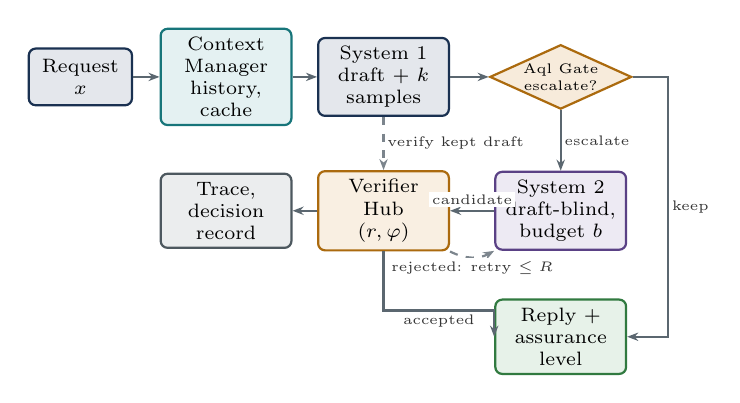
\begin{tikzpicture}[x=1cm,y=1cm]
\node[blk=navy,text width=1.1cm]   (in)  at (0.1,0)    {Request $x$};
\node[blk=teal,text width=1.45cm]   (ctx) at (1.95,0)  {\Mem\\history, cache};
\node[blk=navy,text width=1.45cm]   (s1)  at (3.95,0)  {\Sone\\draft $+$ $k$ samples};
\node[dm,minimum width=1.6cm]      (g)   at (6.2,0)  {\Gate\\escalate?};
\node[blk=violet,text width=1.45cm] (s2)  at (6.2,-1.7) {\Stwo\\draft-blind, budget $b$};
\node[blk=amber,text width=1.45cm]  (v)   at (3.95,-1.7) {\Hub\\$(r,\varphi)$};
\node[blk=slate,text width=1.45cm]  (tr)  at (1.95,-1.7) {Trace, decision record};
\node[blk=leaf,text width=1.45cm]   (out) at (6.2,-3.3) {Reply $+$ assurance level};
\draw[arr] (in)--(ctx); \draw[arr] (ctx)--(s1); \draw[arr] (s1)--(g);
\draw[arr] (g.south)--node[lab,right]{escalate}(s2.north);
\draw[arr] (g.east)--++(0.45,0)|-node[lab,pos=.25,right]{keep}(out.east);
\draw[arr] (s2)--node[lab,above=1pt]{candidate}(v);
\draw[dsh] (v.south east) to[bend right=28] node[lab,below]{rejected: retry $\le R$} (s2.south west);
\draw[arr] (v.south)--++(0,-0.75)-|node[lab,pos=.25,below]{accepted}(out.west);
\draw[dsh] (s1.south)--node[lab,right]{verify kept draft}(v.north);
\draw[arr] (v)--(tr);
\end{tikzpicture}
}
\end{frame}

\begin{frame}{System architecture (single node, CPU)}
\begin{columns}[T]
\column{.6\textwidth}
\centering\scalebox{1.0}{% System architecture (single-node CPU baseline); width ~8.6cm
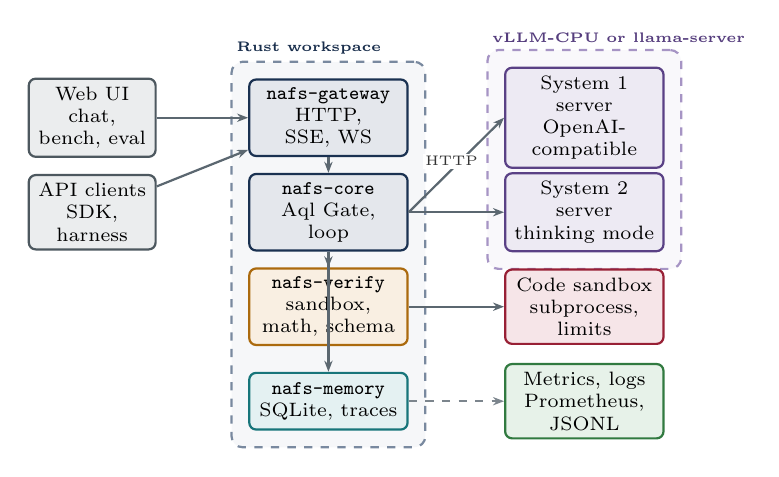
\begin{tikzpicture}[x=1cm,y=1cm]
\node[blk=slate,text width=1.4cm] (ui) at (0.1,0) {Web UI\\chat, bench, eval};
\node[blk=slate,text width=1.4cm] (cli) at (0.1,-1.2) {API clients\\SDK, harness};
\node[blk=navy,text width=1.8cm] (api) at (3.1,0) {\texttt{nafs-gateway}\\HTTP, SSE, WS};
\node[blk=navy,text width=1.8cm] (core) at (3.1,-1.2) {\texttt{nafs-core}\\\Gate, loop};
\node[blk=amber,text width=1.8cm] (hub) at (3.1,-2.4) {\texttt{nafs-verify}\\sandbox, math, schema};
\node[blk=teal,text width=1.8cm] (mem) at (3.1,-3.6) {\texttt{nafs-memory}\\SQLite, traces};
\node[blk=violet,text width=1.8cm] (b1) at (6.35,0) {\Sone\ server\\OpenAI-compatible};
\node[blk=violet,text width=1.8cm] (b2) at (6.35,-1.2) {\Stwo\ server\\thinking mode};
\node[blk=crimson,text width=1.8cm] (sb) at (6.35,-2.4) {Code sandbox\\subprocess, limits};
\node[blk=leaf,text width=1.8cm] (obs) at (6.35,-3.6) {Metrics, logs\\Prometheus, JSONL};
\begin{scope}[on background layer]
\node[grp=navy,fit=(api)(core)(hub)(mem),inner sep=6pt] (gw) {};
\node[grp=violet,fit=(b1)(b2),inner sep=6pt] (srv) {};
\end{scope}
\node[grplab=navy,anchor=south west] at (gw.north west) {Rust workspace};
\node[grplab=violet,anchor=south west] at (srv.north west) {vLLM-CPU or llama-server};
\draw[arr] (ui)--(api); \draw[arr] (cli)--(api);
\draw[arr] (api)--(core); \draw[arr] (core)--(hub); \draw[arr] (core)--(mem);
\draw[arr] (core.east)--node[lab,above,pos=.45]{HTTP}(b1.west);
\draw[arr] (core.east)--(b2.west);
\draw[arr] (hub)--(sb);
\draw[dsh] (mem)--(obs);
\end{tikzpicture}
}
\column{.4\textwidth}
\scriptsize
\begin{itemize}
\item Rust workspace: \texttt{nafs-gateway}, \texttt{nafs-core}, \texttt{nafs-verify}, \texttt{nafs-memory}, \texttt{nafs-web}, \texttt{nafs-eval}, \texttt{nafs-bench}, \texttt{nafs-types}
\item Backends behind one OpenAI-compatible contract: llama-server (macOS, AVX2) or vLLM-CPU (Linux)
\item Every reply: \texttt{reasoning\_mode}, assurance level, decision record
\item GPU scale-out swaps only the model servers
\end{itemize}
\end{columns}
\end{frame}

\begin{frame}{Model profiles (verified on Hugging Face, 2026-10-18)}
\scriptsize
\begin{tabular}{@{}p{1.5cm}p{4.9cm}p{5.2cm}@{}}
\toprule Profile & \Sone & \Stwo\\\midrule
A (reference) & Qwen3-1.7B, Q4\_K\_M 1.3\,GB, thinking off & Qwen3-4B-Thinking-2507, Q4\_K\_M 2.3\,GB\\
B (minimal) & Qwen3-4B, \texttt{enable\_thinking=false} & same weights, thinking on\\
C (upgrade) & Qwen3.5-2B & Qwen3.5-4B (hybrid attention; gate G0 decides)\\
\bottomrule
\end{tabular}
\vspace{2pt}
\begin{columns}[T]
\column{.5\textwidth}
\begin{exampleblock}{Facts that shaped the choice}
\begin{itemize}\item Only Qwen3 and Qwen3.5 have open weights $\le$9B; Qwen3.6/3.8 start at 27B\item Official GGUF exists only for Qwen3; Qwen3-1.7B/4B are on vLLM's validated CPU list\item No official non-autoregressive Qwen exists\end{itemize}
\end{exampleblock}
\column{.5\textwidth}
\begin{alertblock}{Why not Qwen3.5 by default}Hybrid Gated-DeltaNet CPU kernels are newer; vLLM's accelerated path needs AVX-512-BF16 or AMX; no controlled AVX2 benchmark exists. Hypothesis H7 (decode $\ge70\%$ of dense) is measured in Phase~0.\end{alertblock}
\end{columns}
\end{frame}

\section{Stack and feasibility}
\begin{frame}{Implementation stack (verified against current documentation)}
\scriptsize
\begin{columns}[T]
\column{.5\textwidth}
\begin{block}{Serving}
\begin{itemize}\item vLLM: x86 CPU backend needs Linux; AVX-512 recommended, AVX2 limited; AWQ/GPTQ/INT8; pin 0.31.0\item llama-server v0.7.0: GGUF, logprobs, reasoning budget, n-gram speculation; \texttt{n} capped by slots\end{itemize}
\end{block}
\begin{block}{Fine-tuning}Unsloth 2026.10.6 trains only with a GPU; CPU support means inference and data prep. Path: rented 16\,GB GPU, QLoRA (Qwen3) or BF16 LoRA (Qwen3.5), GGUF export, CPU evaluation.\end{block}
\column{.5\textwidth}
\begin{block}{Rust (crates.io, 2026-10-18)}
tokio 1.53, axum 0.8.9, tower-http 0.7, reqwest 0.13, serde, schemars 1.2, utoipa 6.0, sqlx 0.9, tracing, metrics, askama + htmx, figment, criterion, goose.
\end{block}
\begin{exampleblock}{Artefacts}\texttt{openapi.yaml} (two linters), 7 JSON Schemas, vLLM and llama-server configs, Cargo workspace, sample TOML.\end{exampleblock}
\end{columns}
\end{frame}

\begin{frame}{Measured on the reference machine (i3-8100, 4 cores, AVX2, 32\,GB)}
\begin{columns}[T]
\column{.56\textwidth}
\scriptsize
\begin{tabular}{@{}p{3.9cm}rrr@{}}
\toprule Model (GGUF, llama.cpp 797de63) & Size & Prefill & Decode\\\midrule
Qwen3-0.6B Q8\_0 & 604\,MiB & 180.6 & 32.6\\
Qwen3-1.7B Q4\_K\_M & 1.26\,GiB & 94.1 & 15.5\\
Qwen3-4B Q4\_K\_M & 2.32\,GiB & 38.2 & 6.7\\
Qwen3-4B-Thinking-2507 Q4\_K\_M & 2.32\,GiB & 38.4 & 7.0\\
\bottomrule
\end{tabular}
\\[2pt]\scriptsize tokens/s, 4 threads, pp512/tg128, mean of 3 runs; implied bandwidth $\approx$20\,GB/s.
\column{.44\textwidth}\scriptsize
\begin{exampleblock}{Probe (llama-server, Qwen3-1.7B)}logprobs returned; 4 parallel samples in 3.0\,s with 47/48 prompt tokens cached; thinking toggled per request; a 256-token budget closed the trace and an answer followed; SSE streamed.\end{exampleblock}
\begin{alertblock}{Consequence}A 1\,024-token slow reply takes 2--3 min here: demos and batch evaluation, not interactive.\end{alertblock}
\end{columns}
\end{frame}

\section{Specification}
\begin{frame}{Specification highlights (99 requirements, RFC 2119)}
\scriptsize
\begin{columns}[T]
\column{.5\textwidth}
\begin{itemize}
\item \textbf{FR-010--015 Gate:} calibrated $\hat e_1$, per-domain $\hat e_2$, cost ratio; no hand-tuned thresholds in production; failed verification always escalates; decision record per request
\item \textbf{FR-020--026 Deliberation:} sequential verified sampling; $N$, $R$ from the Beta fit; draft-blind; budget forcing; $R\le1$ on non-verifiable tasks; hard caps
\item \textbf{FR-030--035 Verification:} exact verifiers at threshold 1.0; published $(r,\varphi)$; assurance levels; judge hard gate; sandbox limits
\item \textbf{FR-040--042 Ledger:} 5\% audit stream; ``unmeasured'' labels; CUSUM drift
\end{itemize}
\column{.5\textwidth}
\begin{itemize}
\item \textbf{NFR:} wall-clock cap; TTFT $\le2$\,s and 150-token reply $\le12$\,s p95 (fast); slow $\le240$\,s p95 at $b=1024$; $<8$\,GB resident; ECE $\le0.05$; pinned hashes in every trace (targets)
\item \textbf{IF:} OpenAPI 3.1; SSE events \texttt{token/decision/verification/retry/done}; JSON Schemas; backend retry and semaphore policy
\item \textbf{TR:} verified-only data; Unsloth LoRA r=16; GPU path; promotion gate with confidence bounds and human sign-off
\item \textbf{SR:} injection delimiting; sandbox isolation; privacy; analogy-only religious wording with scholar review
\item Traceability matrix: requirement $\to$ result $\to$ component $\to$ test $\to$ phase
\end{itemize}
\end{columns}
\end{frame}

\begin{frame}{Deployment and training pipeline}
\begin{columns}[T]
\column{.5\textwidth}\centering\scalebox{0.5}{% Deployment topology: single-node CPU baseline and optional GPU scale-out; width ~15cm
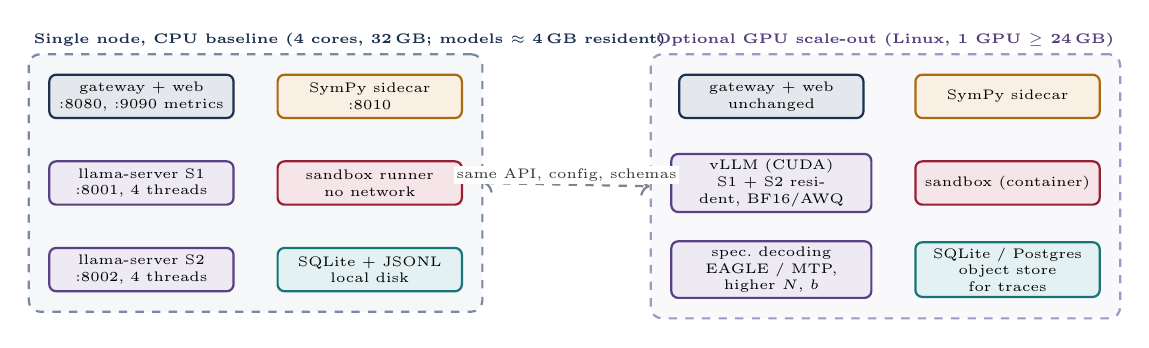
\begin{tikzpicture}[x=1cm,y=1cm]
% CPU node
\node[sblk=navy,text width=2.2cm] (gw) at (0,0) {gateway + web\\:8080, :9090 metrics};
\node[sblk=violet,text width=2.2cm] (s1) at (0,-1.1) {llama-server S1\\:8001, 4 threads};
\node[sblk=violet,text width=2.2cm] (s2) at (0,-2.2) {llama-server S2\\:8002, 4 threads};
\node[sblk=crimson,text width=2.2cm] (sb) at (2.9,-1.1) {sandbox runner\\no network};
\node[sblk=teal,text width=2.2cm] (db) at (2.9,-2.2) {SQLite + JSONL\\local disk};
\node[sblk=amber,text width=2.2cm] (sy) at (2.9,0) {SymPy sidecar\\:8010};
\begin{scope}[on background layer]
\node[grp=navy,fit=(gw)(s1)(s2)(sb)(db)(sy),inner sep=7pt] (cpu) {};
\end{scope}
\node[grplab=navy,anchor=south west] at (cpu.north west) {Single node, CPU baseline (4 cores, 32\,GB; models $\approx$ 4\,GB resident)};
% GPU variant
\node[sblk=navy,text width=2.2cm] (ggw) at (8.0,0) {gateway + web\\unchanged};
\node[sblk=violet,text width=2.4cm] (vl) at (8.0,-1.1) {vLLM (CUDA)\\S1 + S2 resident, BF16/AWQ};
\node[sblk=violet,text width=2.4cm] (vl2) at (8.0,-2.2) {spec.\ decoding\\EAGLE / MTP, higher $N$, $b$};
\node[sblk=crimson,text width=2.2cm] (gsb) at (11.0,-1.1) {sandbox (container)};
\node[sblk=teal,text width=2.2cm] (gdb) at (11.0,-2.2) {SQLite / Postgres\\object store for traces};
\node[sblk=amber,text width=2.2cm] (gsy) at (11.0,0) {SymPy sidecar};
\begin{scope}[on background layer]
\node[grp=violet,fit=(ggw)(vl)(vl2)(gsb)(gdb)(gsy),inner sep=7pt] (gpu) {};
\end{scope}
\node[grplab=violet,anchor=south west] at (gpu.north west) {Optional GPU scale-out (Linux, 1 GPU $\ge$ 24\,GB)};
\draw[dsh,<->] (cpu.east)--node[lab,above]{same API, config, schemas}(gpu.west);
\end{tikzpicture}
}
\column{.5\textwidth}\centering\scalebox{0.78}{% Training (GPU) and serving (CPU) pipeline; width ~8.6cm
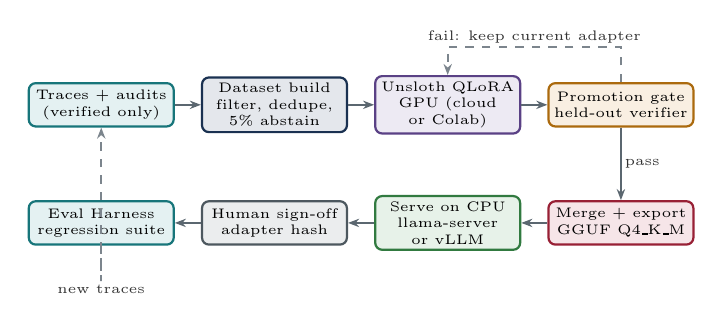
\begin{tikzpicture}[x=1cm,y=1cm]
\node[sblk=teal,text width=1.7cm]   (tr) at (0,0)   {Traces $+$ audits\\(verified only)};
\node[sblk=navy,text width=1.7cm]   (ds) at (2.2,0) {Dataset build\\filter, dedupe, 5\% abstain};
\node[sblk=violet,text width=1.7cm] (ft) at (4.4,0) {Unsloth QLoRA\\GPU (cloud or Colab)};
\node[sblk=amber,text width=1.7cm]  (gate) at (6.6,0) {Promotion gate\\held-out verifier};
\node[sblk=crimson,text width=1.7cm](exp) at (6.6,-1.5) {Merge $+$ export\\GGUF Q4\_K\_M};
\node[sblk=leaf,text width=1.7cm]   (srv) at (4.4,-1.5) {Serve on CPU\\llama-server or vLLM};
\node[sblk=slate,text width=1.7cm]  (hum) at (2.2,-1.5) {Human sign-off\\adapter hash};
\node[sblk=teal,text width=1.7cm]   (ev) at (0,-1.5) {\Harness\\regression suite};
\draw[arr] (tr)--(ds); \draw[arr] (ds)--(ft); \draw[arr] (ft)--(gate);
\draw[arr] (gate)--node[lab,right]{pass}(exp); \draw[arr] (exp)--(srv); \draw[arr] (srv)--(hum);
\draw[arr] (hum)--(ev);
\draw[dsh] (ev.south)--++(0,-0.45)-|node[lab,pos=.25,below]{new traces}(tr.south);
\draw[dsh] (gate.north)--++(0,0.45)-|node[lab,pos=.25,above]{fail: keep current adapter}(ft.north);
\end{tikzpicture}
}
\end{columns}
\vspace{4pt}\small Training runs on a rented GPU; everything else, including the promotion gate and all evaluation, runs on CPU. The GPU scale-out keeps the gateway, verifiers, memory and UI unchanged.
\end{frame}

\section{Roadmap}
\begin{frame}{Eight phases, seven gates (estimates)}
\begin{columns}[T]
\column{.46\textwidth}
\centering\scalebox{0.72}{% Roadmap timeline (weeks); width ~8.6cm; estimates. Phase 7 was added after Phases 0-6 were implemented.
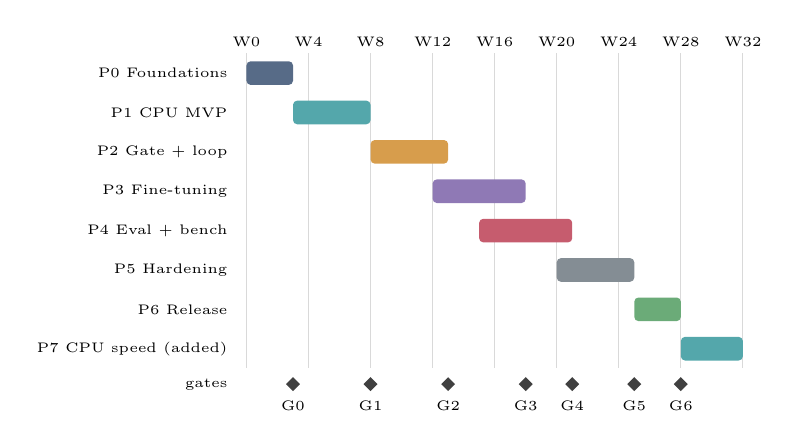
\begin{tikzpicture}[x=0.197cm,y=0.5cm]
\foreach \w in {0,4,...,32}{\draw[black!15] (\w,0.3)--(\w,-7.7);\node[font=\tiny] at (\w,0.6){W\w};}
\foreach \ii/\lbl/\st/\en/\col in {
 0/{P0 Foundations}/0/3/navy,
 1/{P1 CPU MVP}/3/8/teal,
 2/{P2 Gate + loop}/8/13/amber,
 3/{P3 Fine-tuning}/12/18/violet,
 4/{P4 Eval + bench}/15/21/crimson,
 5/{P5 Hardening}/20/25/slate,
 6/{P6 Release}/25/28/leaf,
 7/{P7 CPU speed (added)}/28/32/teal}
 {\node[anchor=east,font=\tiny] at (-0.6,-\ii-0.2){\lbl};
  \fill[\col!75,rounded corners=1.5pt](\st,-\ii-0.5) rectangle (\en,-\ii+0.1);}
\foreach \x/\n in {3/G0,8/G1,13/G2,18/G3,21/G4,25/G5,28/G6}{\node[diamond,fill=black!75,inner sep=1.3pt] (g\n) at (\x,-8.1){};\node[font=\tiny,below=1pt] at (\x,-8.2){\n};}
\node[anchor=east,font=\tiny] at (-0.6,-8.1){gates};
\end{tikzpicture}
}
\column{.54\textwidth}
\scriptsize
\begin{itemize}
\item \textbf{P0} serving, 4\,600-task baseline, verifier rates, H4/H7 \hfill G0
\item \textbf{P1} CPU MVP: gateway, both paths, fixed-rule gate, chat UI \hfill G1
\item \textbf{P2} calibrated gate, verified loop, audits; 3-point non-inferiority \hfill G2
\item \textbf{P3} Unsloth cycle under the promotion gate \hfill G3
\item \textbf{P4} evaluation suite, performance console, drift \hfill G4
\item \textbf{P5} hardening, deployment, optional GPU and Profile~C \hfill G5
\item \textbf{P6} 1-point non-inferiority, scholar review, publication \hfill G6
\item \textbf{P7} CPU inference performance: latency attribution, engine A/B, early escalation, EAGLE-3 (added)
\end{itemize}
61 person-weeks, 42 tasks, every requirement scheduled; backlog exported as CSV and Markdown.
\end{columns}
\end{frame}

\begin{frame}{MVP and critical path}
\begin{columns}[T]
\column{.45\textwidth}
\scriptsize
\begin{block}{MVP (Phase 1)}Profile~A on the reference machine; gateway with chat and SSE; fixed-rule gate with forced escalation on failed verification; code and schema verifiers; draft-blind slow path with budget forcing; assurance levels; decision records; chat UI. Nine acceptance tests (MVP-A1..A9).\end{block}
\begin{alertblock}{Critical path}serving $\to$ baseline $\to$ calibrated gate $\to$ data pipeline $\to$ training $\to$ promotion $\to$ hardening $\to$ release.\end{alertblock}
\column{.55\textwidth}
\centering\scalebox{0.46}{% Dependency and critical-path view (roadmap); width ~15cm
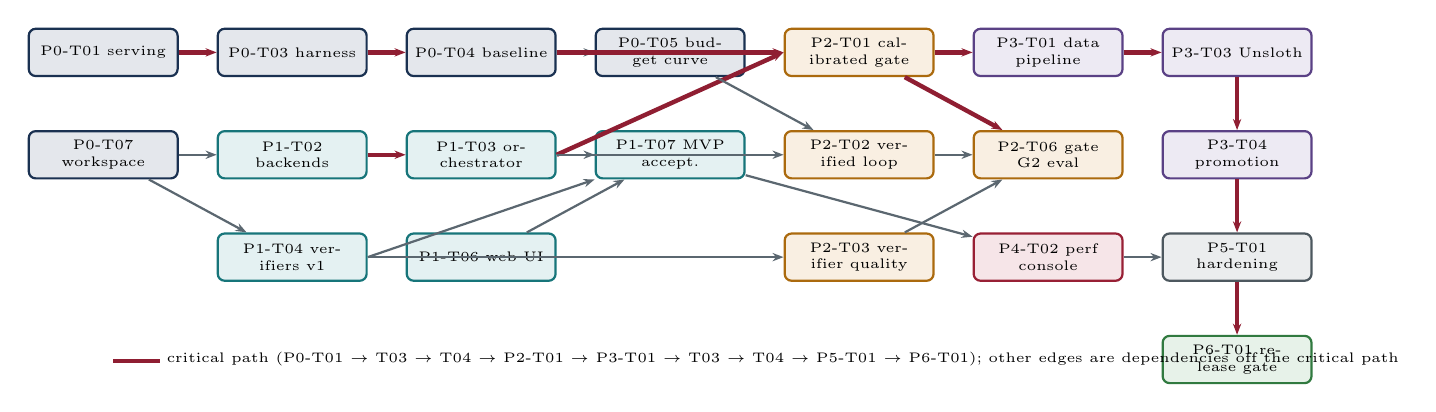
\begin{tikzpicture}[x=1cm,y=1cm]
\tikzset{tk/.style={sblk=#1,text width=1.75cm,minimum height=0.6cm},cp/.style={draw=crimson!80!black,line width=1.6pt}}
\node[tk=navy] (p0t1) at (0,0) {P0-T01 serving};
\node[tk=navy] (p0t3) at (2.4,0) {P0-T03 harness};
\node[tk=navy] (p0t4) at (4.8,0) {P0-T04 baseline};
\node[tk=navy] (p0t5) at (7.2,0) {P0-T05 budget curve};
\node[tk=navy] (p0t7) at (0,-1.3) {P0-T07 workspace};
\node[tk=teal] (p1t2) at (2.4,-1.3) {P1-T02 backends};
\node[tk=teal] (p1t3) at (4.8,-1.3) {P1-T03 orchestrator};
\node[tk=teal] (p1t7) at (7.2,-1.3) {P1-T07 MVP accept.};
\node[tk=teal] (p1t4) at (2.4,-2.6) {P1-T04 verifiers v1};
\node[tk=teal] (p1t6) at (4.8,-2.6) {P1-T06 web UI};
\node[tk=amber] (p2t1) at (9.6,0) {P2-T01 calibrated gate};
\node[tk=amber] (p2t2) at (9.6,-1.3) {P2-T02 verified loop};
\node[tk=amber] (p2t3) at (9.6,-2.6) {P2-T03 verifier quality};
\node[tk=amber] (p2t6) at (12.0,-1.3) {P2-T06 gate G2 eval};
\node[tk=violet] (p3t1) at (12.0,0) {P3-T01 data pipeline};
\node[tk=violet] (p3t3) at (14.4,0) {P3-T03 Unsloth};
\node[tk=violet] (p3t4) at (14.4,-1.3) {P3-T04 promotion};
\node[tk=crimson] (p4t2) at (12.0,-2.6) {P4-T02 perf console};
\node[tk=slate] (p5t1) at (14.4,-2.6) {P5-T01 hardening};
\node[tk=leaf] (p6t1) at (14.4,-3.9) {P6-T01 release gate};
\draw[arr,cp] (p0t1)--(p0t3); \draw[arr,cp] (p0t3)--(p0t4); \draw[arr] (p0t4)--(p0t5);
\draw[arr] (p0t7)--(p1t2); \draw[arr,cp] (p1t2)--(p1t3); \draw[arr] (p1t3)--(p1t7); \draw[arr] (p0t7)--(p1t4); \draw[arr] (p1t4.east)--(p1t7.south west);
\draw[arr] (p1t6)--(p1t7);
\draw[arr,cp] (p0t4)--(p2t1); \draw[arr,cp] (p1t3.east)--(p2t1.west);
\draw[arr] (p1t3.east)--(p2t2.west); \draw[arr] (p0t5)--(p2t2); \draw[arr] (p1t4)--(p2t3);
\draw[arr,cp] (p2t1)--(p2t6); \draw[arr] (p2t2)--(p2t6); \draw[arr] (p2t3)--(p2t6);
\draw[arr,cp] (p2t1)--(p3t1); \draw[arr,cp] (p3t1)--(p3t3); \draw[arr,cp] (p3t3)--(p3t4);
\draw[arr] (p1t7)--(p4t2); \draw[arr] (p4t2)--(p5t1); \draw[arr,cp] (p3t4)--(p5t1); \draw[arr,cp] (p5t1)--(p6t1);
\node[font=\tiny,anchor=west] at (0,-3.9) {\textcolor{crimson!80!black}{\rule{0.6cm}{1.6pt}} critical path (P0-T01 $\to$ T03 $\to$ T04 $\to$ P2-T01 $\to$ P3-T01 $\to$ T03 $\to$ T04 $\to$ P5-T01 $\to$ P6-T01); other edges are dependencies off the critical path};
\end{tikzpicture}
}
\end{columns}
\end{frame}


\section{The system as built}
\begin{frame}{The system as built: chat with an inspectable cascade}
\begin{columns}[T]
\column{.64\textwidth}
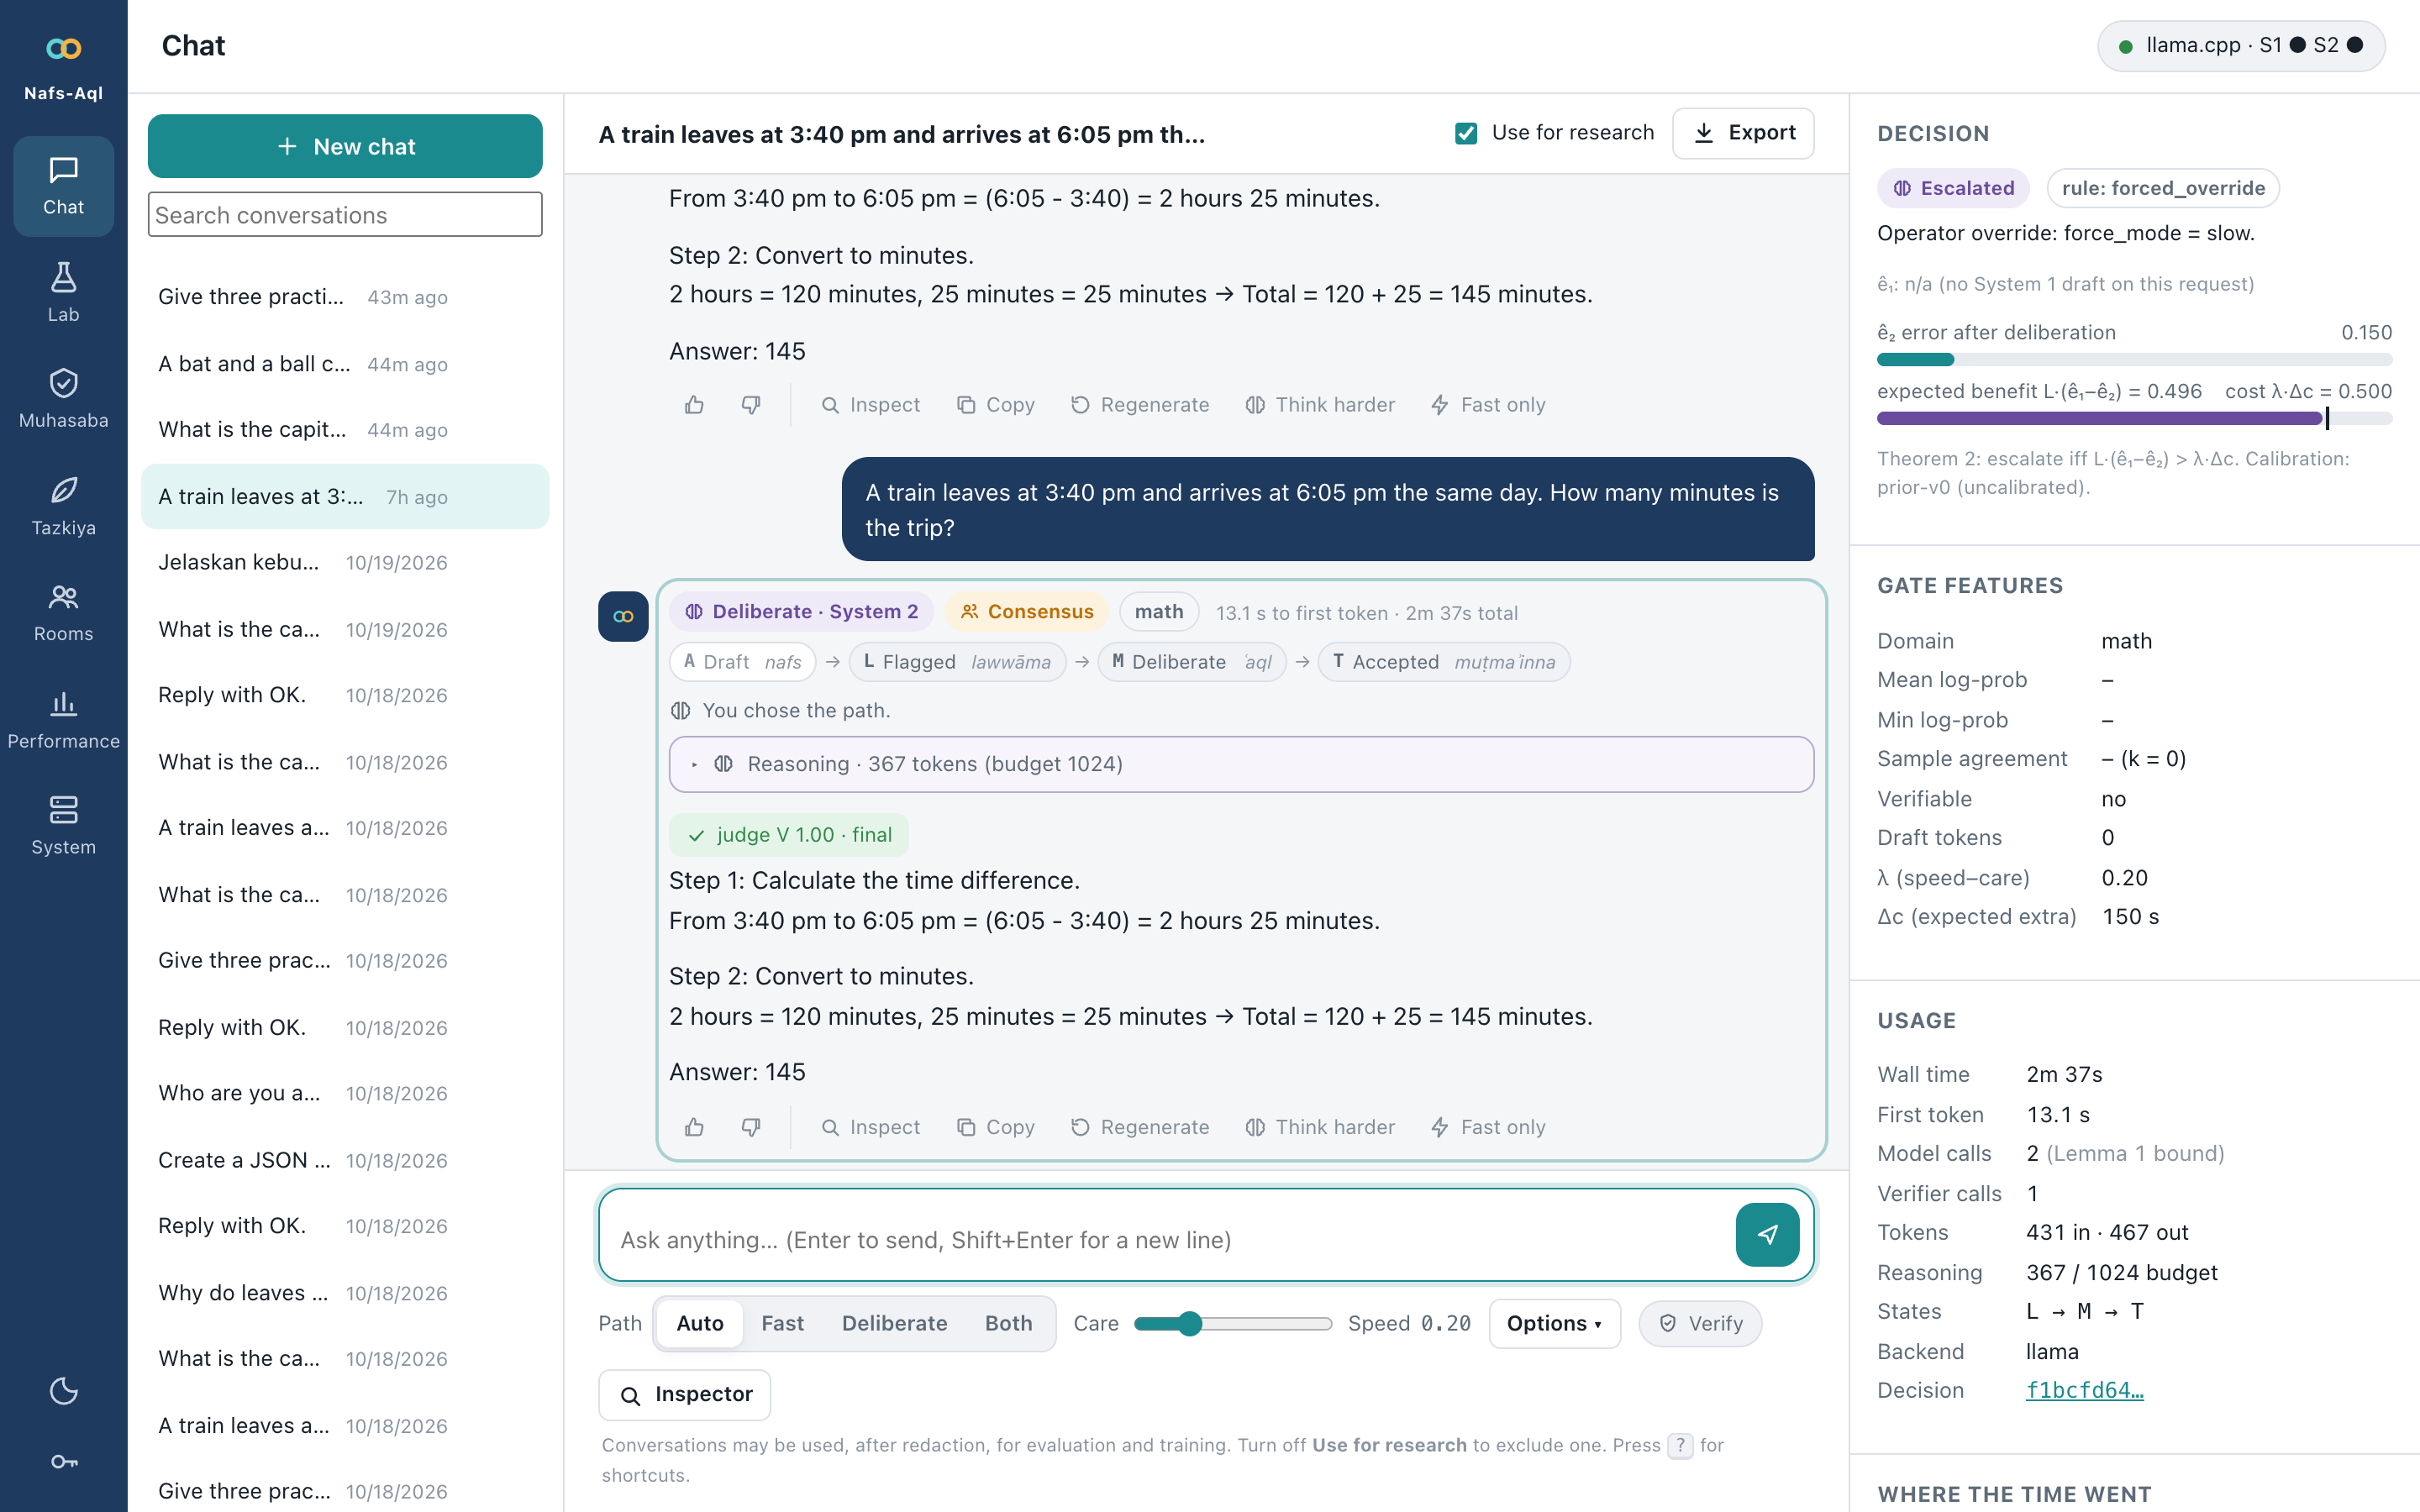
\includegraphics[width=\linewidth]{../shared/screenshots/chat.png}
\column{.36\textwidth}
\scriptsize
\begin{itemize}
\item Rust workspace of 8 crates; 50 documented endpoints (OpenAPI 1.5); OpenAI-compatible chat
\item System~1 Qwen3-1.7B, System~2 Qwen3-4B-Thinking-2507, Q4\_K\_M on llama-server (vLLM-CPU profile in a VM)
\item Each answer shows the strip A$\to$L$\to$M$\to$T/X, its assurance and the gate's reason; the inspector shows the decision, features and a per-stage latency waterfall
\item Here: the draft passed the code tests, so the gate kept it (Theorem~1)
\item \emph{Both} trials: a person compares System~1 and System~2 answers on the same prompt
\end{itemize}
\end{columns}
\end{frame}

\begin{frame}{The laboratory: when should System 2 be consulted?}
\begin{columns}[T]
\column{.6\textwidth}
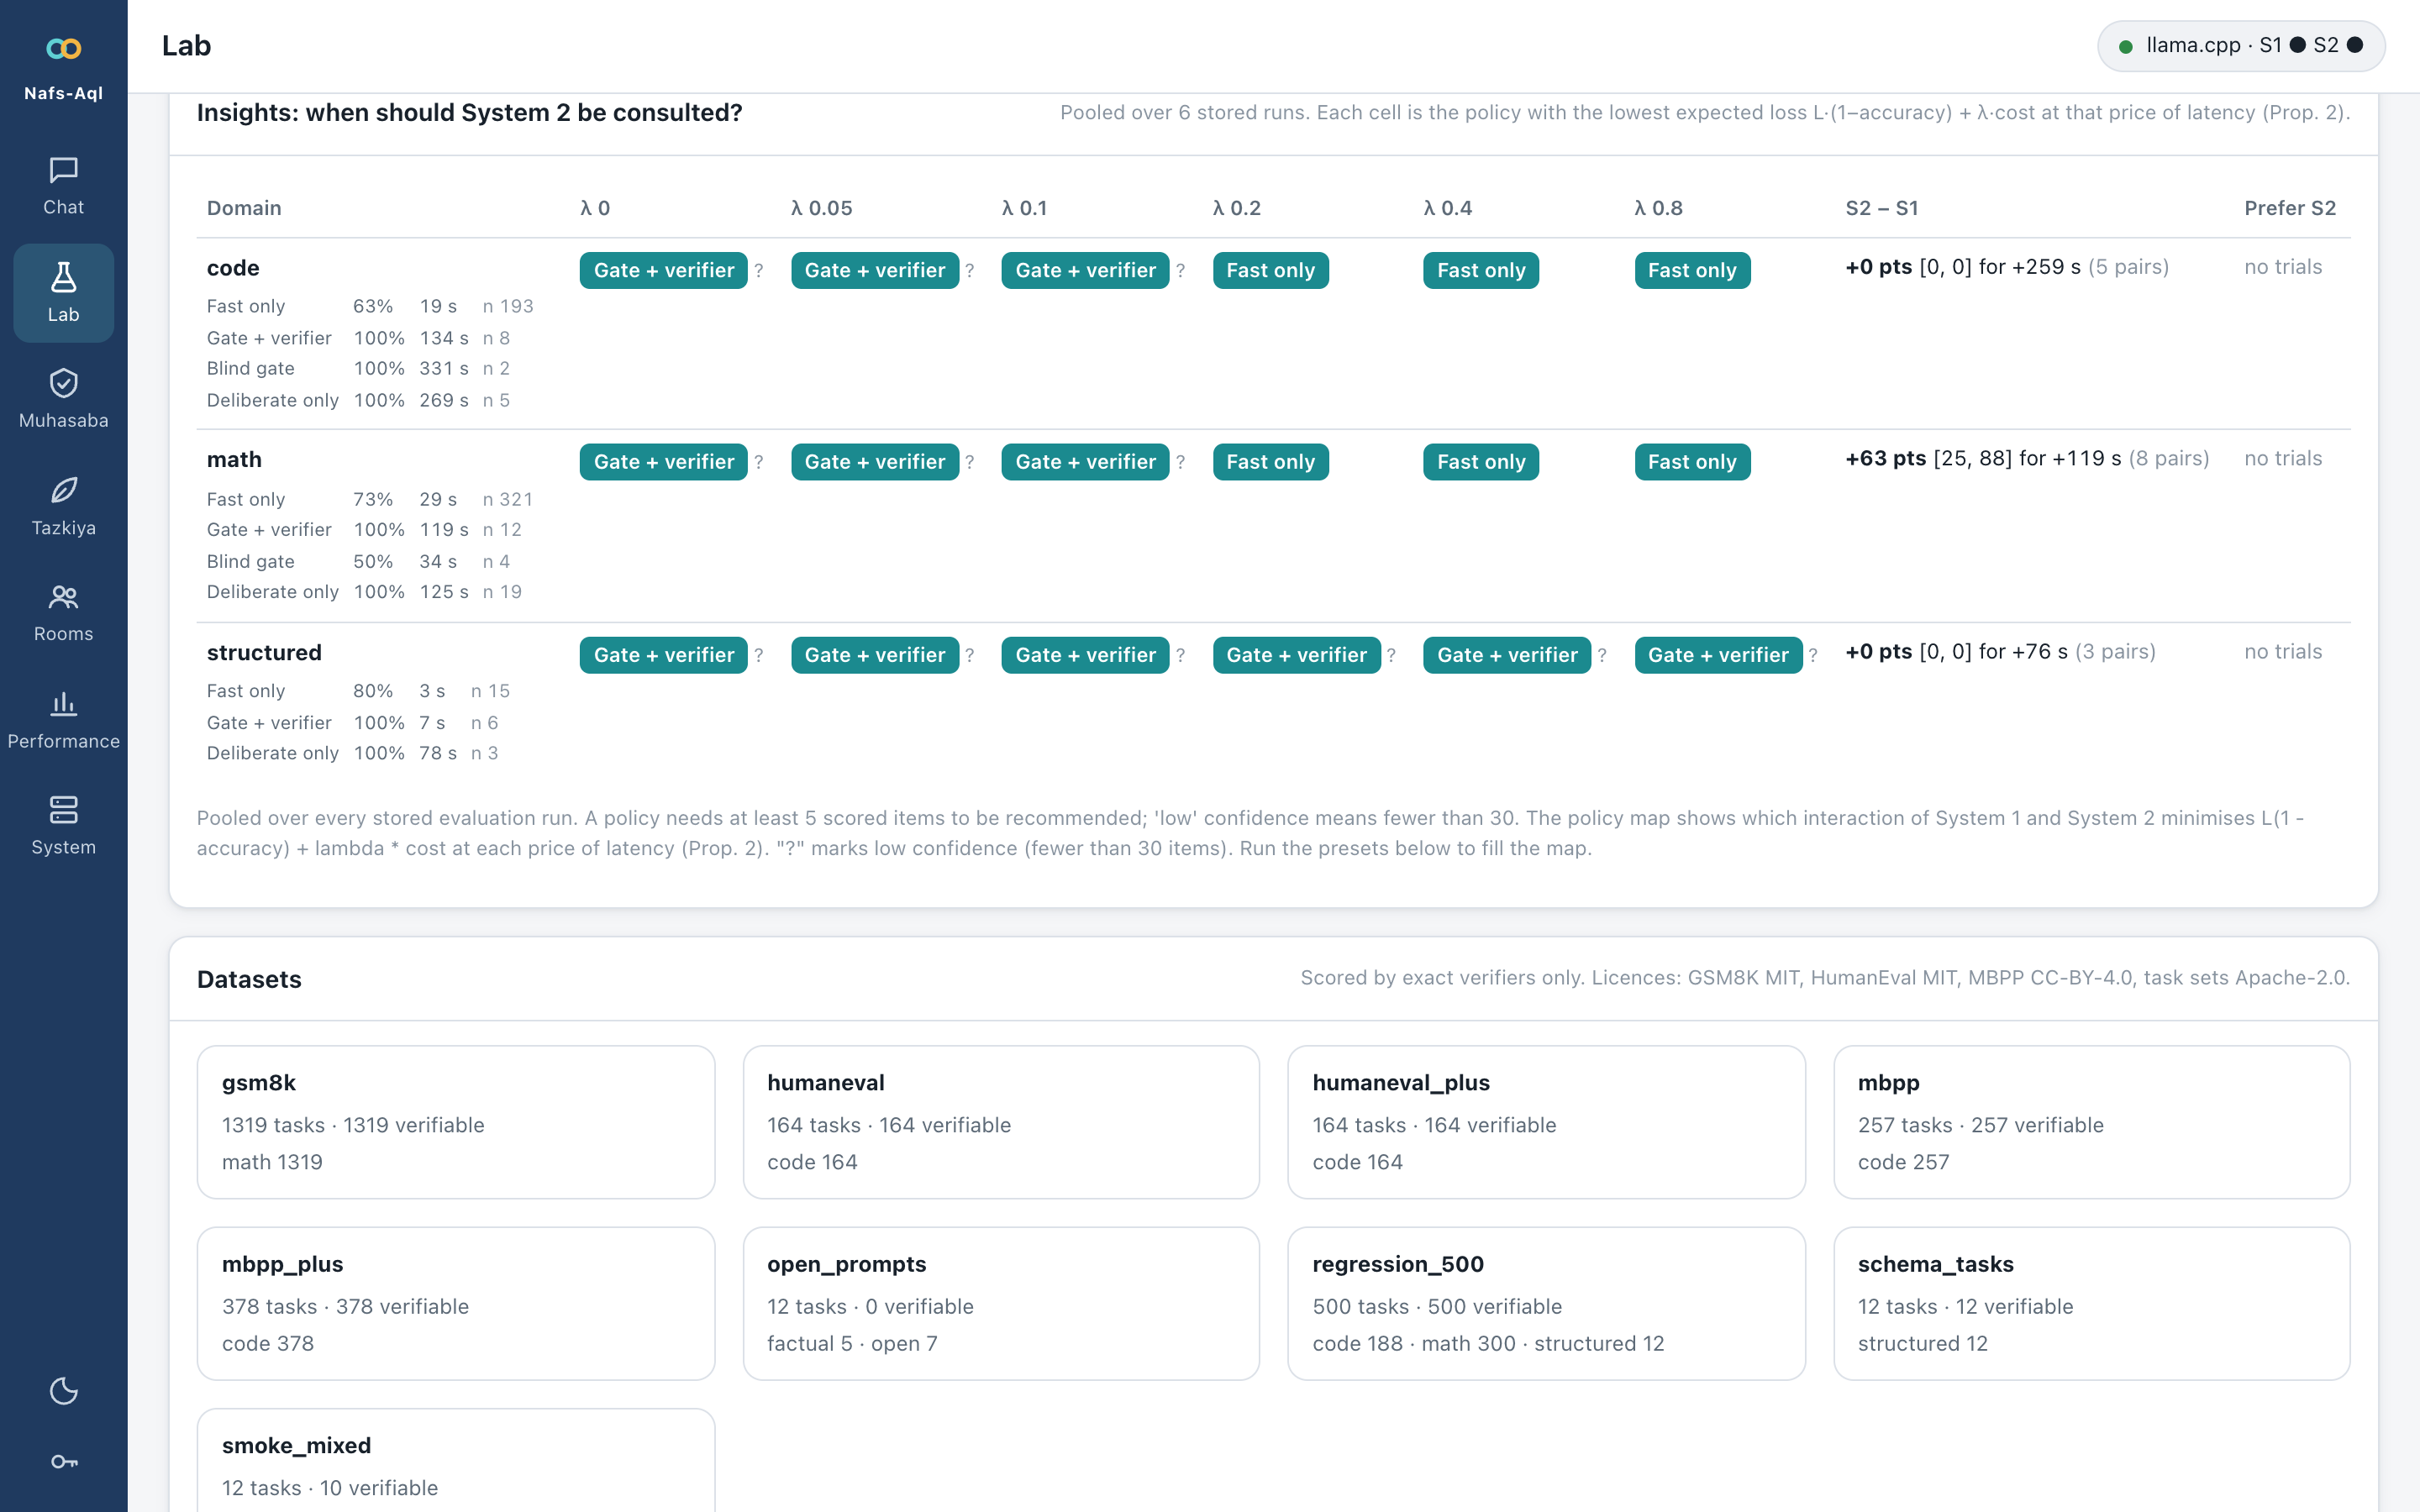
\includegraphics[width=\linewidth]{../shared/screenshots/lab_insights.png}
\column{.4\textwidth}
\scriptsize
\begin{itemize}
\item Each combination of the two systems is a \emph{policy}: fast only, deliberate only, gate with verifier, blind gate, draft-conditioned ablation, budget and $\lambda$ sweeps
\item The policy map pools every run: per domain and price of latency $\lambda$, the policy with the lowest $L(1-\mathrm{acc})+\lambda c$
\item Now (\PolicyMapRuns{} runs): \PolicyMapSummary
\item Paired bootstrap CIs, exact McNemar, Bonferroni; exports to Markdown and CSV
\end{itemize}
\end{columns}
\end{frame}

\begin{frame}{Measured results (indicative)}
\begin{columns}[T]
\column{.5\textwidth}
\scriptsize\textbf{Policies} (run \PhaseTwoRun)\par
\resizebox{\linewidth}{!}{\PhaseTwoTable}\par\medskip
Gate with verifier = deliberate-only accuracy at \GatedCostRatio{} of the cost; the blind gate routed \BlindRouting{} correctly (samples agreed with wrong drafts).
\column{.5\textwidth}
\scriptsize\textbf{Verifiers} ($r$ true accept, $\varphi$ false accept)\par
\resizebox{\linewidth}{!}{\VerifierTable}\par\medskip
\textbf{Profile~C} (System~1 candidates, 30 tasks)\par
\resizebox{\linewidth}{!}{\ProfileCTable}\par
Qwen3.5-2B: \ProfileCDelta, but 3.7$\times$ slower $\Rightarrow$ Profile~A stays.
\end{columns}
\end{frame}

\begin{frame}{Phase 7: where the time goes on a CPU}
\begin{columns}[T]
\column{.55\textwidth}
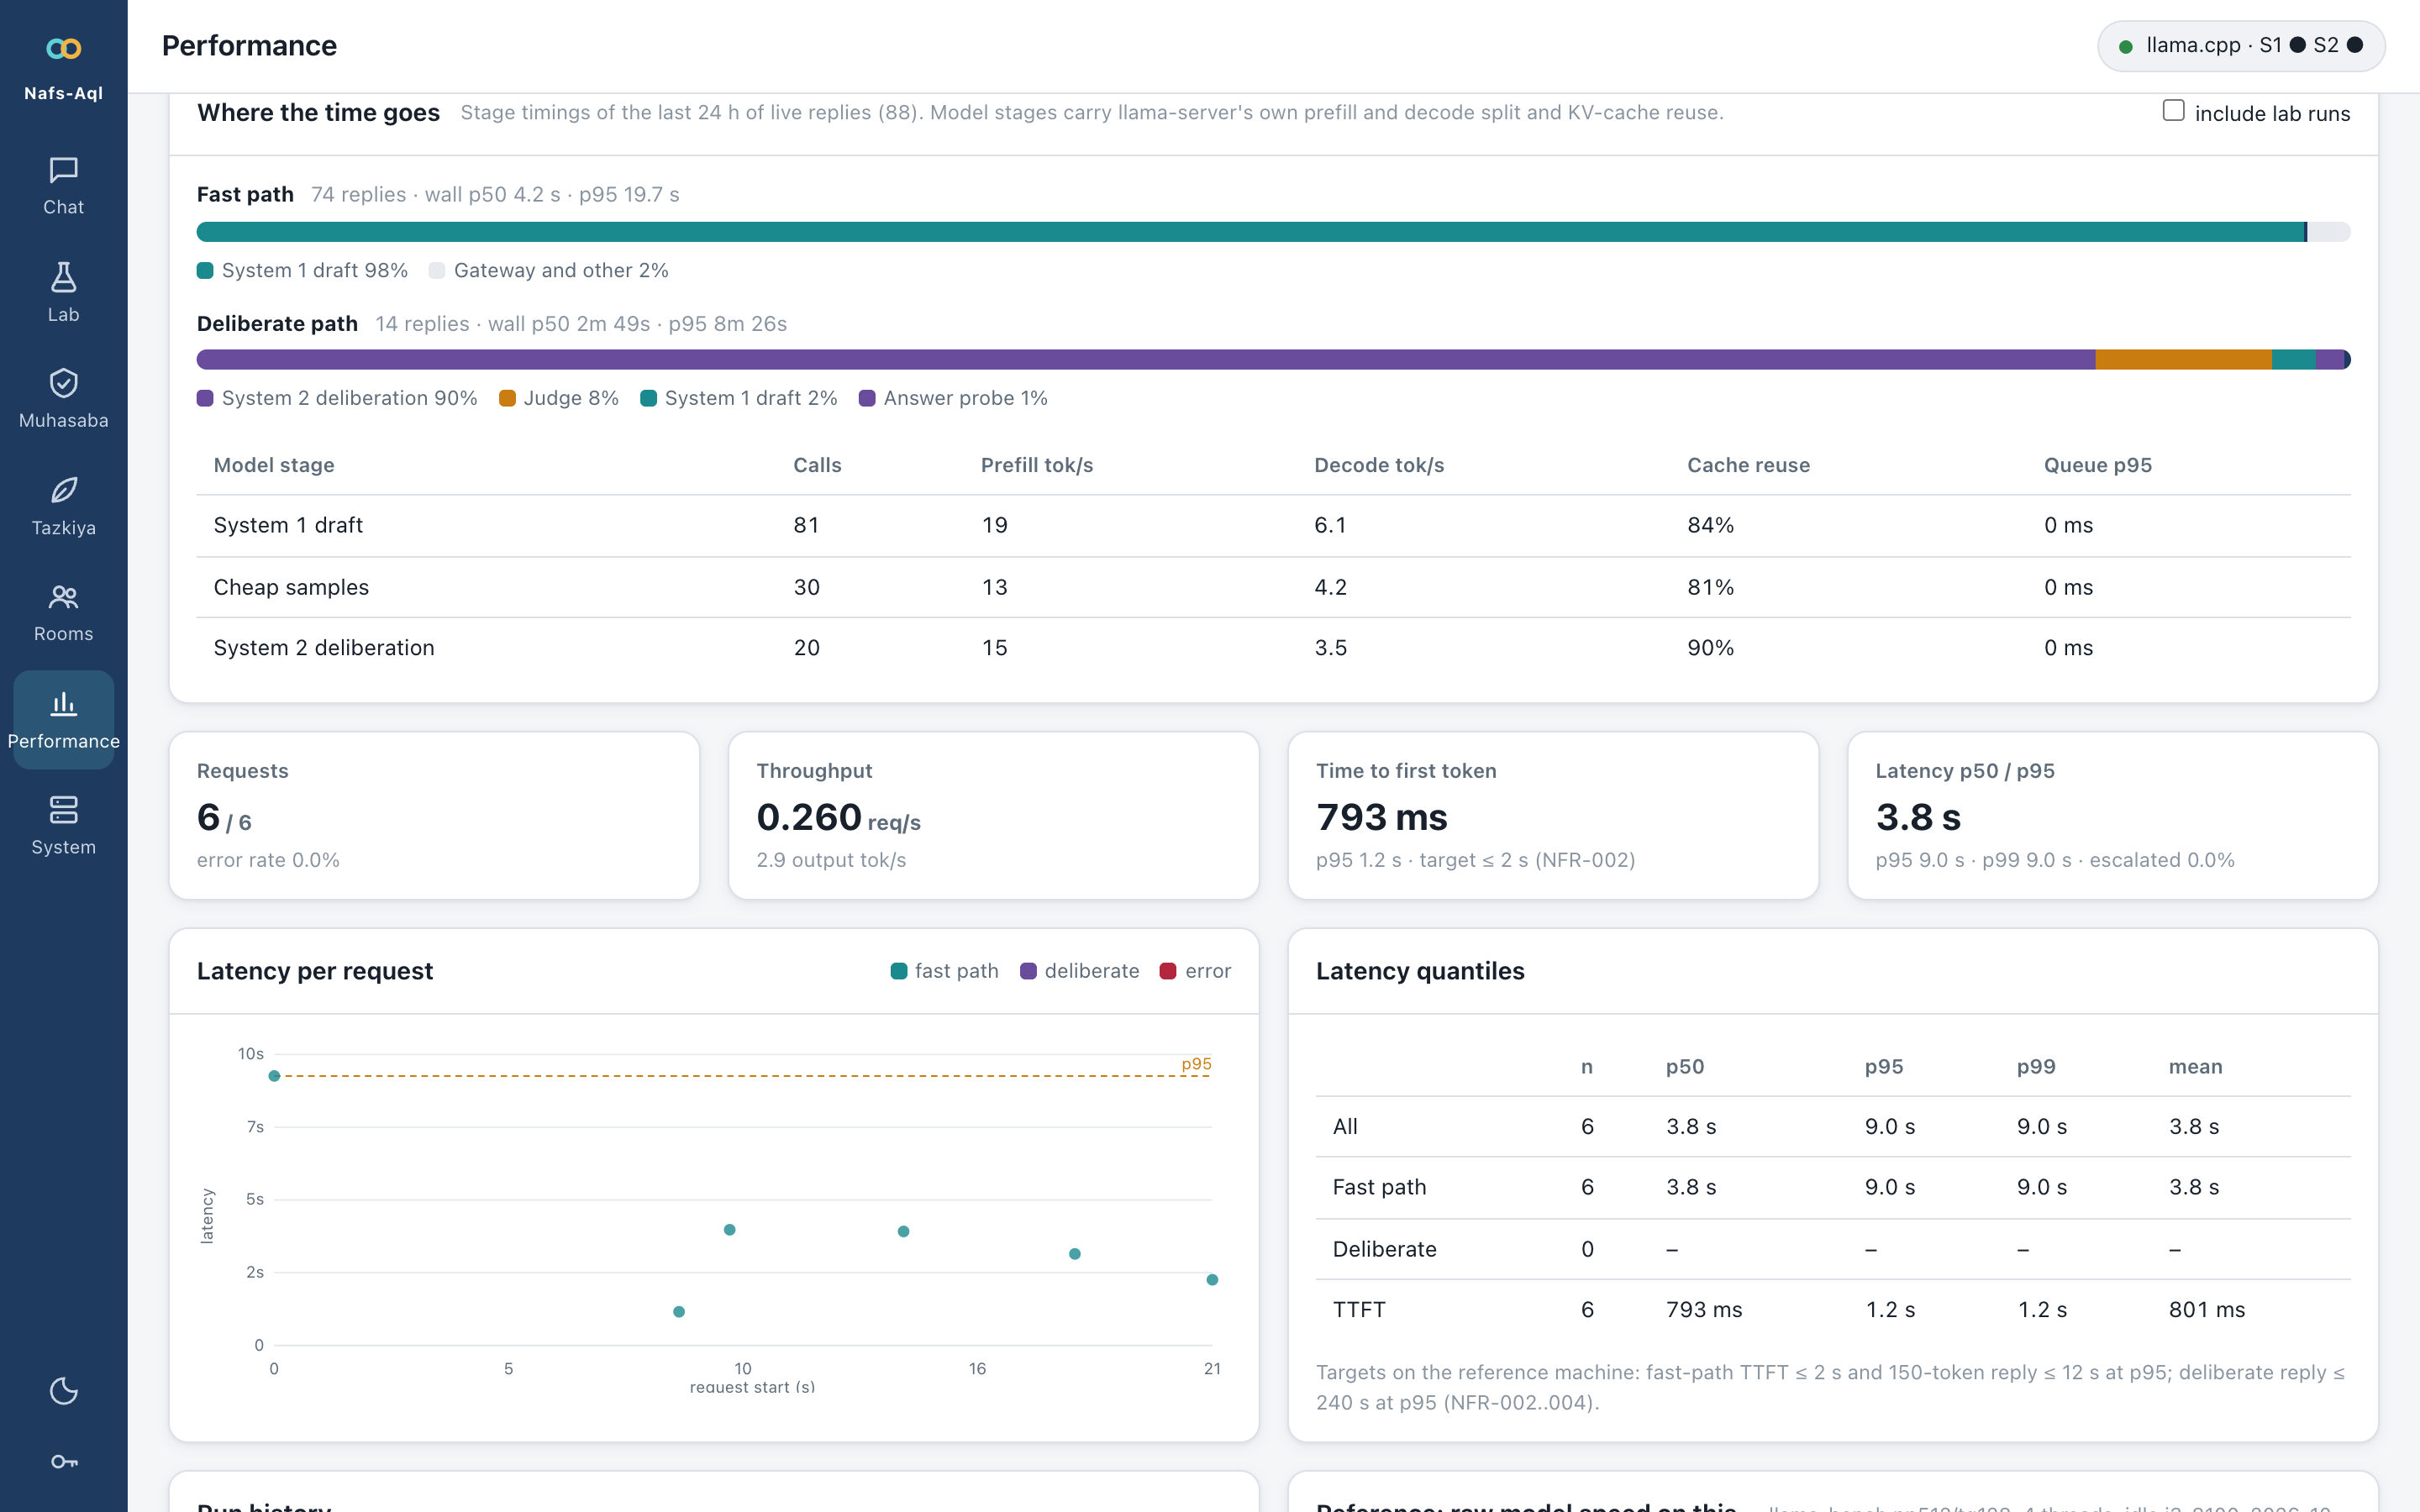
\includegraphics[width=\linewidth]{../shared/screenshots/performance_stages.png}
\column{.45\textwidth}
\scriptsize
\begin{itemize}
\item Every reply records its stages; model stages carry llama-server's prefill, decode and KV-cache reuse
\item Fast path $\approx$100\% System~1 draft; deliberate path $\approx$97\% System~2 reasoning; the prompt cache serves most prompt tokens $\Rightarrow$ \textbf{decode speed is the bottleneck}
\item Shared host: 2.6--4.3 tok/s in service vs 22.9 idle
\end{itemize}
\resizebox{\linewidth}{!}{\EngineTable}
\begin{exampleblock}{Adopted after interleaved A/B}
Skip samples when a verifier decides (13.4$\to$7.9\,s); samples only when the draft is uncertain (factual 12.6$\to$4.3\,s); prompt-cache and verifier warm-up (TTFT 9.8$\to$1\,s); early escalation; 4 System~1 slots
\end{exampleblock}
\end{columns}
\end{frame}

\begin{frame}{Early escalation, concurrency, and the next engine levers}
\begin{columns}[T]
\column{.5\textwidth}
\scriptsize
\begin{block}{Early escalation (FR-080)}
Stop an open-ended draft once its running mean log-prob is below the fixed threshold minus a margin; System~2 takes over. 40 prompts: N\,=\,32, margin 0.04 agrees 100\%, catches 3/10 escalations, saves $\approx$116 tokens each.
\end{block}
\centering\resizebox{0.92\linewidth}{!}{\EarlyEscTable}
\column{.5\textwidth}
\scriptsize
\begin{block}{Concurrency (NFR-007)}
Latest protocol run \ProtocolRun: ratio \NfrSevenRatio. Gate G4 uses the median over eligible runs: \NfrSevenPooled.
\end{block}
\begin{exampleblock}{Adaptive reasoning exit (FR-082, new)}
System~2 reasons in chunks; at reflection points its answer is probed and the exact verifier decides whether to stop. Paired Lab run: \AdaptiveExitSummary.
\end{exampleblock}
\begin{alertblock}{Measured, no gain, not adopted}
0.6B draft and n-gram speculation; flash attention, q8\_0 KV; EAGLE-3 heads (1.04$\times$ / 0.99$\times$); System~1 as judge ($\varphi$ 0.27 vs 0.045).
\end{alertblock}
\end{columns}
\end{frame}

\begin{frame}{Backends and weight formats: measured, not assumed}
\begin{columns}[T]
\column{.5\textwidth}
\scriptsize
\begin{block}{vLLM CPU backend in Docker (new)}
\texttt{carstenz/vllm-smoke} image (vLLM 0.30, x86 CPU build), one model in two modes on :8101; the gateway switches backend sets at run time.
\begin{itemize}
\item AVX2-only VM: BF16 loads but never returns a token (no oneDNN kernels) $\Rightarrow$ FP32
\item vLLM's three processes cost $\approx$3\,GB beyond the weights: 1.7B needs an 11--12\,GiB VM, 0.6B about 7
\item Gateway check (every orchestrator path): \VllmCheckSummary
\end{itemize}
\end{block}
\column{.5\textwidth}
\scriptsize
\begin{block}{Weight formats (llama-bench, Qwen3-1.7B)}
\centering\resizebox{0.7\linewidth}{!}{\QuantTable}\par
The repack formats buy nothing over Q4\_K\_M on AVX2; the format stays.
\end{block}
\begin{block}{A smaller judge?}
\JudgeCompare. Accepting a quarter of wrong answers is not a verifier (Thm.\,1): the judge stays on System~2.
\end{block}
\end{columns}
\end{frame}

\begin{frame}{Muhasaba: drift, alerts, security and the gates}
\begin{columns}[T]
\column{.5\textwidth}
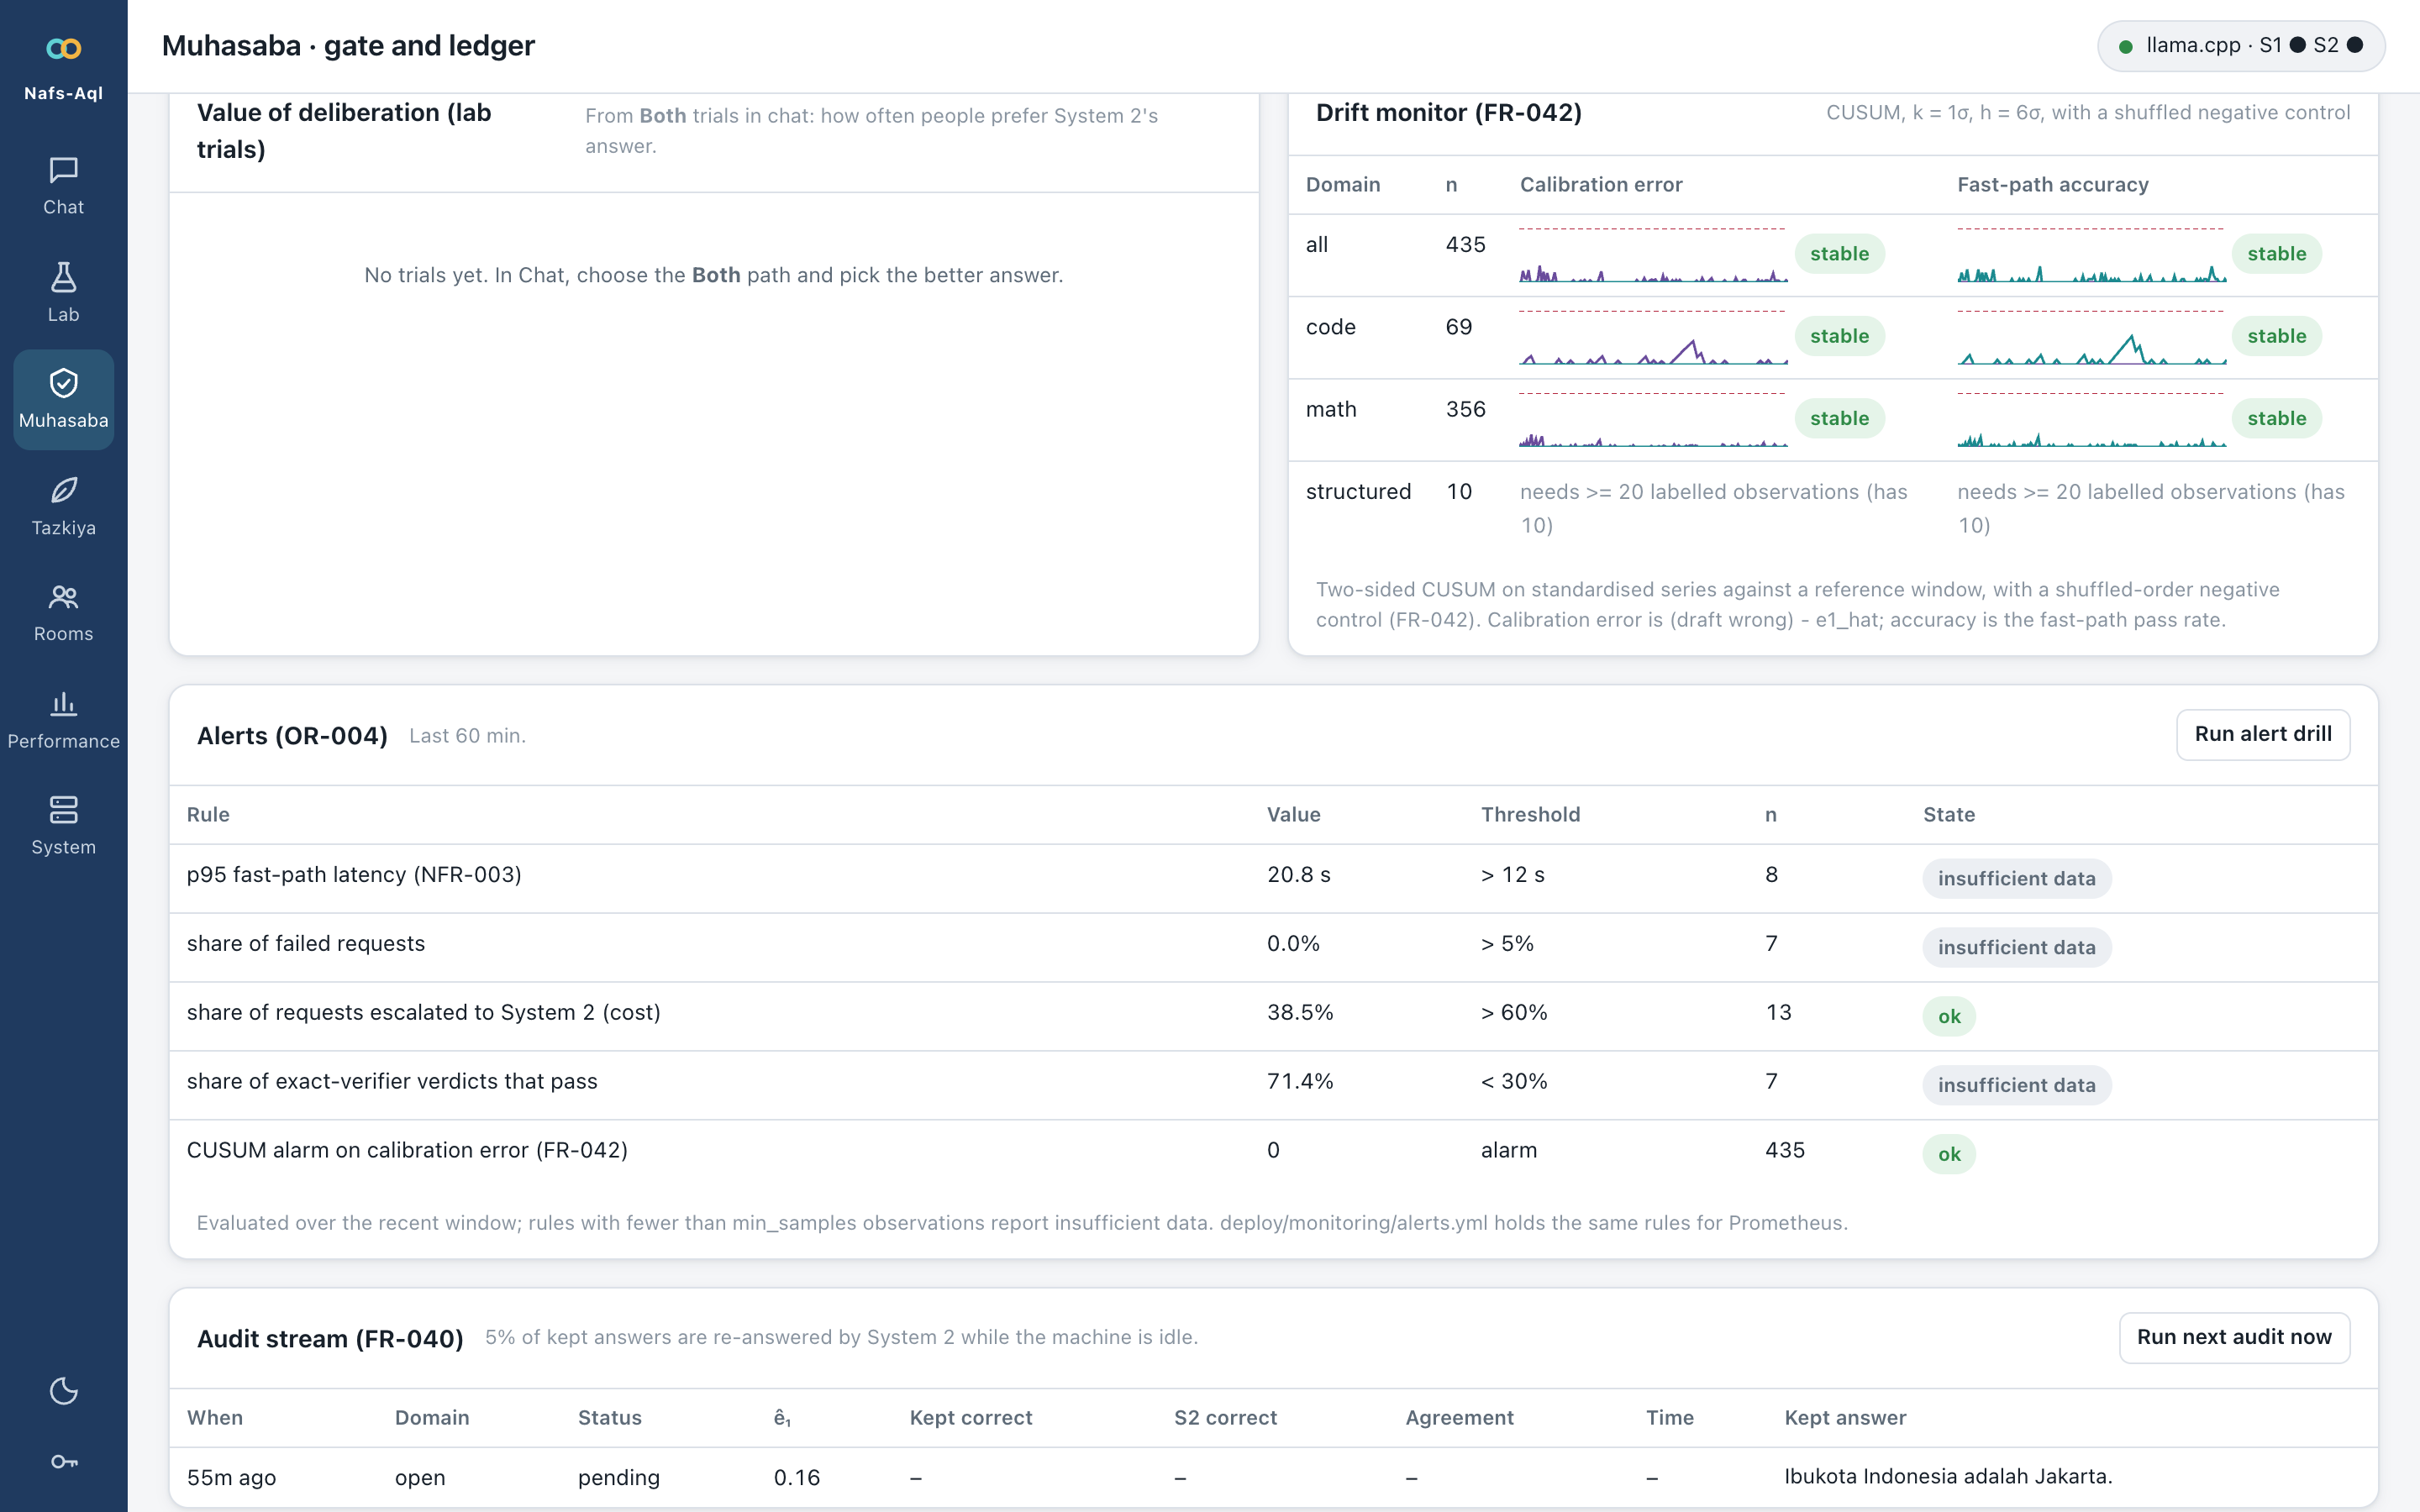
\includegraphics[width=\linewidth]{../shared/screenshots/muhasaba_drift_alerts.png}
\scriptsize
CUSUM drift per domain with a shuffled negative control; five alert rules over live traffic (lab traffic tagged). \SecuritySummary; deployment checks: \DeploySummary.
\column{.5\textwidth}
\centering\resizebox{\linewidth}{!}{\GatesTable}
\end{columns}
\end{frame}

\section{Evaluation}
\begin{frame}{Evaluation plan and statistically sized gates}
\begin{columns}[T]
\column{.5\textwidth}
\scriptsize
\begin{itemize}
\item \textbf{Metrics:} accuracy, selective accuracy and coverage, escalation rate, routing accuracy vs the oracle rule, cost ratio and cost--accuracy curve, ECE (5 bins, $n\ge2\,900$), verifier $(r,\varphi)$ with intervals, adoption rate, robustness, latency quantiles
\item \textbf{Benchmarks:} GSM8K, MATH, HumanEval, MBPP, schema tasks, MMLU, GPQA, TruthfulQA, SimpleQA, BBH, LiveCodeBench, MT-Bench style; RouteLLM data for calibration
\item \textbf{Protocol:} paired, seeded, bootstrap CIs, non-inferiority (3 points at G2, 1 point at G6), Bonferroni across domains, CUSUM drift with negative control
\end{itemize}
\column{.5\textwidth}
\centering\scalebox{0.78}{% Evaluation workflow; width ~8.6cm
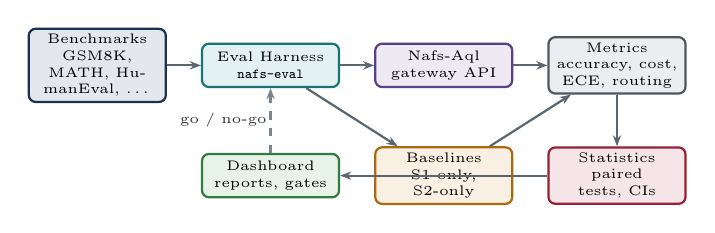
\begin{tikzpicture}[x=1cm,y=1cm]
\node[sblk=navy,text width=1.6cm]   (ds) at (0,0)    {Benchmarks\\GSM8K, MATH, HumanEval, \ldots};
\node[sblk=teal,text width=1.6cm]   (h)  at (2.2,0)  {\Harness\\\texttt{nafs-eval}};
\node[sblk=violet,text width=1.6cm] (sys) at (4.4,0) {\Sys\\gateway API};
\node[sblk=amber,text width=1.6cm]  (bl) at (4.4,-1.4) {Baselines\\S1-only, S2-only};
\node[sblk=slate,text width=1.6cm]  (m)  at (6.6,0)  {Metrics\\accuracy, cost, ECE, routing};
\node[sblk=crimson,text width=1.6cm](st) at (6.6,-1.4) {Statistics\\paired tests, CIs};
\node[sblk=leaf,text width=1.6cm]   (db) at (2.2,-1.4) {Dashboard\\reports, gates};
\draw[arr] (ds)--(h); \draw[arr] (h)--(sys); \draw[arr] (h)--(bl); \draw[arr] (sys)--(m); \draw[arr] (bl)--(m);
\draw[arr] (m)--(st); \draw[arr] (st)--(db); \draw[dsh] (db)--node[lab,left]{go / no-go}(h);
\end{tikzpicture}
}
\vspace{2pt}\scriptsize
\begin{block}{Hypotheses H1--H7}Gate accuracy; cost ratio; Beta fit; concave budget curve; coupling; distillation gain; hybrid CPU speed. Each has an experiment, a phase and an engineering effect if false.\end{block}
\end{columns}
\end{frame}

\begin{frame}{Risks, assumptions, and the first three actions}
\scriptsize
\begin{columns}[T]
\column{.5\textwidth}
\begin{alertblock}{Top risks}
\begin{itemize}\item Slow path not interactive on CPU (mitigate: smaller budget, Profile~B, GPU profile)\item Gate calibration may fail on uninformative features (budget mode, richer features)\item Verifier false accepts (hidden tests, mutation testing)\item Correlated errors across shared weights (exact verifiers carry the case)\item Version drift of models and runtimes (pins, hashes, regression suite)\end{itemize}
\end{alertblock}
\column{.5\textwidth}
\begin{block}{Key assumptions}CPU-only means the i3-8100 class; Unsloth runs on a rented GPU; vLLM on Linux, llama-server elsewhere, same API; the draft's missing companion documents are inferred from the deck.\end{block}
\begin{exampleblock}{First three actions}
\begin{enumerate}\item Run the Phase-0 baseline ($\ge4\,600$ tasks) and fit $e_1$, $e_2$, Beta, budget curves \emph{(harness done; only scaled runs on this CPU)}\item Mutation-test the code, math and schema verifiers; publish $(r,\varphi)$ \emph{(done)}\item llama-bench Qwen3.5-2B/4B vs Qwen3-1.7B/4B on the target CPU \emph{(done: H7 passes; Profile~C not adopted)}\end{enumerate}
\end{exampleblock}
\end{columns}
\end{frame}

\begin{frame}{The road ahead (beyond Phase 7)}
\scriptsize
\begin{columns}[T]
\column{.5\textwidth}
\begin{block}{Phase 8: evidence at scale}
Faster or idle host (or nightly slices): the 4\,600-task baseline, 700 paired items for G2, 2\,900 labelled drafts to promote the calibrated gate and budget mode, 6\,200 pairs for G6.
\end{block}
\begin{block}{Phase 9: Tazkiya cycle}
5\,000 verified traces, the first Unsloth LoRA on a rented GPU, promotion under TR-007, rollback drill; re-fit the EAGLE-3 head to the distilled System~1.
\end{block}
\column{.5\textwidth}
\begin{block}{Phase 10: engine}
EAGLE-3 / MTP speculation; repacked 4-bit formats; adaptive early exit from System~2 reasoning; a learned router from the policy map and Both-trial preferences.
\end{block}
\begin{block}{Phase 11: product and review}
Scholar review of the analogy text (SR-005); GPU profile for interactive deliberation; multilingual UI (Indonesian, Arabic); open-domain evidence checks from retrieval.
\end{block}
\end{columns}
\end{frame}

\begin{frame}[standout]
Nafs-Aql: deliberate when it pays, accept only on evidence, keep honest accounts.
\end{frame}
\end{document}
